\documentclass[twoside]{iisthesis}
\usepackage[MeX]{polski}
\usepackage[cp1250]{inputenc}
\usepackage{graphicx}
\usepackage{cite}
\usepackage{xcolor}
\usepackage{epstopdf}
\usepackage{tablefootnote}
\usepackage{siunitx}
\usepackage{booktabs}

% definicje kolorow
\definecolor{ciemnoSzary}{rgb}{0.15,0.15,0.15}
\definecolor{szary}{rgb}{0.5,0.5,0.5}
\definecolor{jasnoSzary}{rgb}{0.2,0.2,0.2}
\newcommand\todo[1]{\textcolor{red}{#1}}

\begin{document}

% Zmiana domy�lnych angielskich nazw cz�ci dokumentu na polskie "Rozdzia�y s� w klasie issthesis"
% wst�pnie poprawione mo�e kto� b�dzie zna� lepszy spos�b i wrzuci to do klasy issthesis.cls
\renewcommand{\contentsname}{Spis tre�ci}
\renewcommand{\appendixname}{Dodatek}
\renewcommand{\listfigurename}{Spis ilustracji}
\renewcommand{\listtablename}{Spis tabel}
\renewcommand{\refname}{Bibliografia}
\renewcommand{\abstractname}{Streszczenie}

\title{Predykcja defekt�w na poziomie metod w celu zredukowania wysi�ku zwi�zanego z zapewnieniem jako�ci oprogramowania}
\author{Mateusz Kutyba}
\advisor{dr hab. in�. Lech Madeyski}
\instituteLogo{logos/pwr}
\slowaKluczowe{predykcja defekt�w\\metryki oprogramowania\\oceny oparte na wysi�ku}

\date{\number\the\year}

% Wstawienie streszczenia pracy
\abstractSH{Przewidywanie b��d�w w oprogramowaniu z wykorzystaniem algorytm�w uczenia maszynowego, na podstawie metryk oprogramowania i danych historycznych. \newline \newline}
\abstractPL{Streszczenie po polsku}
\abstractEN{Abctract in english}

%spis tre�ci
\maketitle
\textpages

%%%%%%%%%%%%%%%%%%%%%%%%%%%%%%%%%%%%%%%%%%%%%%%%%%%%%%%%%%%%
\chapter{Wst�p}
\label{rozdzial1}
\noindent
Prawdopodobnie nie istniej� programy wolne od b��d�w. Z~ca�� pewno�ci� istniej� programy, kt�re zawieraj� zbyt du�� liczb� b��d�w. Ka�dy kto tworzy oprogramowanie chcia�by aby by�o ono wolne od wad. Podstawowym narz�dziem pozwalaj�cym na sprawdzenie czy program dzia�a poprawnie s� testy. Powstaj� coraz bardziej wyszukane metody i~metodyki testowania oprogramowania, a~wszystko po to aby oprogramowanie dzia�a�o zgodnie z~oczekiwaniami, czyli aby cechowa�o si� wysok� jako�ci�. Testowanie i~inspekcje kodu pozwalaj� zapewni� odpowiedni� jako�� oprogramowania, ale s� kosztowne. Bazuj�c na zasadzie Pareto \cite{endres2003handbook} wiemy, �e oko�o 80\% defekt�w pochodzi z~20\% modu��w \cite{concas2011distribution}. Wiedz�c, kt�re modu�y nale�y podda� inspekcji, mo�na znacznie obni�y� ilo�� pracy potrzebn� do znalezienia wi�kszo�ci b��d�w, a~co za tym idzie znacz�co zmniejszy� koszt takich inspekcji.

Kod �r�d�owy oprogramowania zazwyczaj sk�ada si� z~wielu plik�w, kt�re s� organizowane w~pakiety (ang. \textit{packages}). W~j�zyku Java pliki zawieraj� klasy (ang. \textit{class}), a~ka�da klasa mo�e zawiera� metody (ang. \textit{method}). Powsta�o wiele metod predykcji defekt�w, na r�nych poziowach granulacji: od pakiet�w, przez pliki, klasy, metody, na pojedynczych zmianach (ang. \textit{hunk} \cite{ferzund2009empirical, ferzund2009software}) sko�czywszy \cite{hall2012systematic, catal2009systematic, d2010extensive, d2012evaluating}. Jak wykazano m.in. w~\cite{giger2012method} i~\cite{hata2012bug}, predykcja b��d�w na poziomie metod dostarcza dok�adniejszych danych na temat lokalizacji b��d�w, dzi�ki czemu ich odnajdywanie jest efektywniejsze.

Predykcja defekt�w oprogramowania wykorzystuje techniki eksploracji danych, g��wnie s� to metody statystyczne i~metody uczenia maszynowego. Kluczowym elementem w~tych procesach s� w�a�nie dane. To na ich podstawie algorytmy uczenia maszynowego s� w~stanie formu�owa� regu�y decyzyjne. W~in�ynierii oprogramowania tymi danymi s� r�znego rodzaju metryki oprogramowania. Podzia� metryk oraz ich zastosowanie zosta�y szerzej opisane w~rozdziale \ref{rola-metryk}.

Gromadzenie danych (metryk) z~projekt�w jest czasoch�onne, wymaga du�o pracy --- pobierania lub kopiowania projekt�w, mocy obliczeniowej do wyliczenia metryk. Potrzebne jest stworzenie uniwersalnych rozwi�za� s�u��cych do tego celu oraz nastawienie na mo�liwo�� rozszerzania zestawu narz�dzi, kt�re mog� by� ze sob� dowolnie zestawiane. Te wymagania spe�nia platforma DePress \cite{madeyski2014software}, kt�ra jest rozwijana przy udziale student�w i~pracownik�w Politechniki Wroc�awskiej oraz pracownik�w Capgemini Polska. Wi�cej informacji o~DePress zawarto w~rozdziale \ref{depress}.

Wst�pne przeszukiwanie literatury wykaza�o niewielk� ilo�� �r�de� �ci�le odpowiadaj�cych zagadnieniu predykcji defekt�w na niskim poziomie granulacji. Jest to g��wny kierunek tych bada� a~ich celem jest przede wszystkim opracowanie nowego modelu, kt�ry mia�by s�u�y� do efektywnego wskazywania miejsc w~oprogramowaniu, w~kt�rych znajduj� si� b��dy. Pozwololi�oby to na ograniczenie ilo�ci pracy potrzebnej do przejrzenia krytycznych miejsc i~naprawienia b��d�w.





%%%%%%%%%%%%%%%%%%%%%%%%%%%%%%%%%%%%%%%%%%%%%%%%%%%%%%%%%%%%
%%%%%%%%%%%%%%%%%%%%%%%%%%%%%%%%%%%%%%%%%%%%%%%%%%%%%%%%%%%%
\section{Cele pracy}

\noindent Cele pracy dyplomowej:
\begin{itemize}
	\item Przegl�d literatury pod k�tem predykcji defekt�w oprogramowania, szczeg�lnie na niskim poziomie granulacji.
	\item Budowa nowych lub rozbudowa istniej�cych narz�dzi s�u��cych do wyliczenia metryk oprogramowania, wsp�pracuj�cych z~wersjonowanymi repozytoriami kodu (wsparcie dla Git).
	\item Zebranie danych z~projekt�w o~otwartych �r�d�ach na potrzeby predykcji defekt�w.
	\item Budowa modeli predykcji z~wykorzystaniem zebranych danych.
	\item Ocena stworzonych narz�dzi oraz zebranych danych.
	\item Ewaluacja modeli predykcji i~ocena ich skuteczno�ci.
\end{itemize}





%%%%%%%%%%%%%%%%%%%%%%%%%%%%%%%%%%%%%%%%%%%%%%%%%%%%%%%%%%%%
\subsection{Przeznaczenie narz�dzi}

\noindent Narz�dzia stworzone w~ramach pracy dyplomowej wchodz� w~sk�ad platformy (ang. \textit{framework}) DePress\footnote{http://depress.io} (\textit{Defect Prediction in Software Systems}). Jest to rozszerzalna platforma pozwalaj�ca na budowanie przep�ywu pracy (ang. \textit{workflow}) w~spos�b graficzny, dzi�ki temu, �e jest oparta na projekcie KNIME. G��wnym celem DePress jest wspieranie analizy empirycznej oprogramowania. Pozwala na zbieranie, ��czenie i~analiz� danych z~r�nych �r�de�, jak repozytoria oprogramowania czy metryki.






%%%%%%%%%%%%%%%%%%%%%%%%%%%%%%%%%%%%%%%%%%%%%%%%%%%%%%%%%%%%
\subsection{Ograniczenia dotycz�ce realizacji}

\noindent Poni�ej wypisano ograniczenia dotycz�ce realizacji bada�:
\begin{itemize}
	\item badanie tylko projekt�w o~otwartych �r�d�ach (ang. \textit{open source}),
	\item badanie tylko projekt�w napisanych w~j�zyku Java,
	\item wykorzystanie narz�dzi platformy DePress, lub stworzenie nowych narz�dzi w~ramach platformy,
	\item mo�liwo�� �atwego, najlepiej zautomatyzowanego powt�rzenia badania,
	\item wykorzystanie j�zyka R~do budowy modeli predykcji defekt�w.
\end{itemize}








%%%%%%%%%%%%%%%%%%%%%%%%%%%%%%%%%%%%%%%%%%%%%%%%%%%%%%%%%%%%
\subsection{Metoda oceny}

\noindent Podstawow� ocen� efektywno�ci tworzonych modeli by�a ocena oparta na wysi�ku (ang. \textit{effort-based evaluation}). Dla ka�dego modelu zosta�a stworzona krzywa efektywno�ci, przyk�ad takiej krzywej przedstawia rysunek \ref{example-chart}. Por�wnanie efektywno�ci modeli polega przede wszystkim na por�wnaniu procentowej ilo�ci b��d�w znalezionych w~okre�lonej ilo�ci kodu. Przyj�to, �� warto�ci� graniczn� kodu poddanego inspekcji b�dzie 20\%. Taka sama warto�� jest stosowana w~innych badaniach. W~przedstawionym przyk�adzie dokonuj�c przegl�du 20\% kodu, znajdzie si� w~nim 30\% encji z~defektami (w~przypadku tych bada� s� to metody).

\begin{figure}[htbp]
	\caption{Wykres krzywej efektywno�ci}
	\label{example-chart}
	\centering
	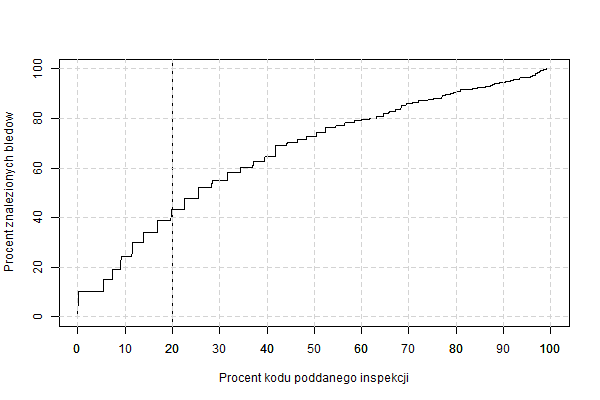
\includegraphics[width=.75\textwidth]{charts/example}
\end{figure}

Dodatkowo zastosowano inne miary skuteczno�ci klasyfikator�w, w~nawiasie zawarto symbol kt�rym s� oznaczane:
\begin{itemize}
	\item dok�adno�� ($A$),
	\item wsp�czynnik Kappa Cohena ($\kappa$),
	\item powierzchnia pod krzyw� ROC ($AUC$).
\end{itemize}

\paragraph{Dok�adno��,} ang. \textit{Accuracy}, $A$. Jest to stosunek poprawnie sklasyfikowanych instancji do wszystkich instancji. Maksymalna dok�adno�� wynosz�ca 1 oznacza ca�kowit� zgodno�� wyniku predykcji z~rzeczywistymi klasami. Minimalna warto�� to 0.
\begin{equation}
	A=\frac{TP+TN}{TP+TN+FP+FN}
\end{equation}

\paragraph{Wsp�czynnik Kappa Cohena,} $\kappa$. Jest miar� statystyczn� okre�laj�c� zgodno�� pomi�dzy r�nymi klasyfikatorami. Bierze pod uwag� przypadkow� zgodno��, dzi�ki czemu mo�na okre�li� czy dok�adno�� przewy�sza poziom losowej dok�adno�ci. Wsp�czynnik sprawdza si� dobrze w~problemach gdzie liczno�� instancji w~poszczeg�lnych klasach nie jest r�wna. Maksymalna warto�� Kappa to 1 a~minimalna to -1.
\begin{equation}
	\kappa=\frac{A-RA}{1-RA} \qquad \textrm{gdzie } RA=\frac{(TP+FN)(TP+FP)+(TN+FP)(TN+FN)}{(TP+TN+FP+FN)^{2}}
\end{equation}

\paragraph{Powierzchnia pod krzyw� ROC,} ang. \textit{Area Under the Curve}, $AUC$. Klasyfikatory nie okre�laj� samej przynale�no�ci do klasy, ale warto�� prawdopodobie�stwa z~jakim dana instancja nale�y do danej klasy. Daje to mo�liwo�� wykre�lenia krzywej zale�no�ci pomi�dzy TP i~FP. Krzywa na wykresie okre�lana jest jako ROC (ang. \textit{Receiver Operating Characteristic}). Pole pod t� krzyw� reprezentuje skuteczno�� klasyfikatora. Idealny klasyfikator uzyska wynik 1, natomiast losowy klasyfikator powinien uzyska� wynik 0,5. Wykres \ref{example-roc} przedstawia przyk�ad krzywej ROC.
\begin{figure}[htbp]
	\caption{Wykres krzywej ROC}
	\label{example-roc}
	\centering
	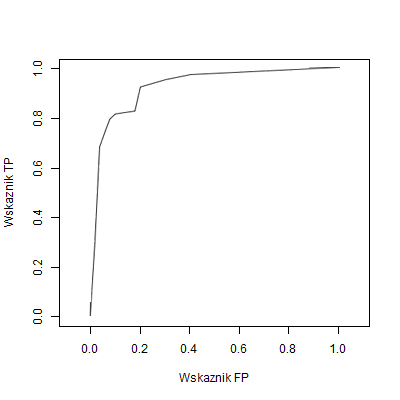
\includegraphics[width=.5\textwidth]{charts/example-roc}
\end{figure}








%%%%%%%%%%%%%%%%%%%%%%%%%%%%%%%%%%%%%%%%%%%%%%%%%%%%%%%%%%%%
%%%%%%%%%%%%%%%%%%%%%%%%%%%%%%%%%%%%%%%%%%%%%%%%%%%%%%%%%%%%
\section{Struktura pracy}

\noindent Dalsza cz�� pracy zosta�a podzielona w~nast�puj�cy spos�b. W~rozdziale \ref{rozdzial2} opisano przegl�d literatury oraz om�wiono aktualny stan wiedzy. W~rozdziale \ref{rozdzial3} zawarto charakterystyk� wykorzystanych narz�dzi, oprogramowania i~j�zyk�w. W~rozdziale \ref{rozdzial4} opisano przebieg bada� i~ich wyniki, natomiast w~rozdziale \ref{rozdzial5} przeanalizowano uzyskane rezultaty, podsumowano badanie pod k�tem jego potencjalnego zastosowania i~mo�liwo�ci dalszego rozwoju. Rozdzia� ten zawiera r�wnie� istotny fragment dotycz�cy zagro�e� dla wiarygodno�ci przeprowadzonego badania.


%%%%%%%%%%%%%%%%%%%%%%%%%%%%%%%%%%%%%%%%%%%%%%%%%%%%%%%%%%%%
\chapter{Przegl�d literatury}
\label{rozdzial2}
\noindent
%%%%%%%%%%%%%%%%%%%%%%%%%%%%%%%%%%%%%%%%%%%%%%%%%%%%%%%%%%%%
%%%%%%%%%%%%%%%%%%%%%%%%%%%%%%%%%%%%%%%%%%%%%%%%%%%%%%%%%%%%
\section{Zwi�zek z~innymi pracami}

\noindent Na pocz�tku prac dokonano przegl�du literatury aby okre�li� aktualny stan wiedzy (ang. \textit{state of the art}) w~badanej dziedzinie. Przegl�d literatury pozwoli� udzieli� odpowiedzi na nast�puj�ce pytania:
\begin{itemize}
	\item {\bf Jakie istniej� metody predykcji defekt�w na poziomie metod i~jaka jest ich skuteczno��?}
		\\Istnieje wiele modeli predykcji defekt�w, jednak wi�kszo�� z~nich opiera si� na danych dotycz�cych klas, pakiet�w lub modu��w. Odpowiedzi� na powy�sze pytanie jest zbi�r modeli predykcji defekt�w na niskim poziomie granulacji, na przyk�ad metod lub blok�w kodu.
	\item {\bf Jakie s� mo�liwo�ci usprawnienia lub rozwini�cia istniej�cych metod?}
		\\Zosta�y zebrane wszelkie mo�liwo�ci ulepszenia lub rozszerzenia bada� wskazanych przez autor�w, okre�lone np. jako ``Dalszy rozw�j".
	\item {\bf Jakie s� sposoby ekstrakcji zmian kodu �r�d�owego na poziomie metod?}
		\\Jakie s� sposoby por�wnywania wersji kodu �r�d�owego, jakiego rodzaju dane (metryki) s� uzyskiwane.
\end{itemize}

Podczas wst�pnego rozpoznania dziedziny zauwa�ono, �e liczba publikacji jest niewielka. W~zwi�zku z~tym postanowiono przeprowadzi� wyszukiwanie w~dw�ch etapach. W~pierwszym etapie przeszukano elektroniczne zbiory, natomiast w~drugim etapie przejrzano bibliografie pozyskanych publikacji a~tak�e wszystkie publikacje ich autor�w w~celu odnalezienia dodatkowych tekst�w.

\paragraph{Przeszukiwalne zbiory cyfrowe.}

Przeszukano poni�sze zbiory z~u�yciem ustalonych wyra�e�, za pomoc� wyszukiwarek udost�pnianych w~postaci aplikacji internetowej:
\begin{itemize}
	\item IEEE Xplore,
	\item Science Direct,
	\item ACM Digital Library,
	\item Springer Link,
	\item ISI Web of Science.
\end{itemize}

Wybrano te zbiory poniewa� pokrywaj� one wi�kszo�� publikacji in�ynierii oprogramowania oraz s� u�ywane jako �r�d�a w~innych przegl�dach z~tej dziedziny \cite{hall2012systematic, riaz2009systematic}.



W celu przygotowania listy wyra�e� u�ytych do przeszukiwania zbior�w podj�to nast�puj�ce kroki:
\begin{enumerate}
	\item Przet�umaczenie pyta� na j�zyk angielski.
		\begin{itemize}
			\item What are the methods to predict defects on method level and what is their efficiency?
			\item What are the possibilities to improve or extend existing methods?
			\item What are the methods to extract source code changes on method level?
		\end{itemize}
	\item Wypisanie s��w kluczowych dotycz�cych pyta� badawczych.
		\begin{itemize}
			\item defect prediction, method level, efficiency, extract, source changes, code changes
		\end{itemize}

	\item Wypisanie synonim�w i alternatywnych form.
		\begin{itemize}
			\item bug prediction, fault prediction, detection, fine granularity, fine-grained, performance, code metrics, process metrics, software evolution
		\end{itemize}

	\item Utworzenie form z gwiazdk� (*) zast�puj�cych liczb� pojedyncz� i mnog� oraz alternatywne formy i ko�c�wki.
		\begin{itemize}
			\item bug, fault, defect*, predict*, detect*
			\item method level, fine, grain*
			\item efficien*, performance
			\item code, process, metric*, change*, software, evolution
		\end{itemize}

	\item Wykonanie pr�bnego przeszukiwania a nast�pnie wybranie s��w kluczowych ze znalezionych trafnych wynik�w (brano pod uwag� s�owa kluczowe oraz streszczenie).

	\item Przygotowanie z�o�onych zapyta� wykorzystuj�c dost�pne operatory:
		\begin{itemize}
			\item {\bf IEEE Xplore}:
				\begin{itemize}
					\item ((bug OR fault OR defect*) AND (predict* OR detect*)) AND ((method NEAR level) OR (fine AND grain*))
					\item ((code OR process) AND metric*) AND ((``Abstract":bug OR ``Abstract":fault OR ``Abstract":defect*) AND (``Abstract":predict* OR ``Abstract":detect*)) AND (``Abstract":efficien* OR ``Abstract":performance)
					\item ((source NEAR code) AND change*) AND ((method NEAR level) OR (fine AND grain*))
				\end{itemize}

			\item {\bf Science Direct} (w kategorii Computer Science):
				\begin{itemize}
					\item title-abstr-key(((bug OR fault OR defect*) AND (predict* OR detect*)) AND ((method W/1 level) OR (fine W/1 grain*)))
					\item title-abstr-key(((input AND data) OR ((code OR process) AND metric*)) AND ((bug OR fault OR defect*) AND (predict* OR detect*)) AND (efficien* OR performance))
					\item title-abstr-key((source AND code AND change*) AND ((method AND level) OR (fine AND grain*)))
				\end{itemize}

			\item {\bf ACM Digital Library}:
				\begin{itemize}
					\item ((bug OR fault OR defect*) AND (predict* OR detect*)) AND ((method AND level) OR (fine AND grain*))
					\item ((input AND data) OR ((code OR process) AND metric*)) AND ((bug OR fault OR defect*) AND (predict* OR detect*)) AND (efficien* OR performance)
					\item (source AND code AND change*) AND ((method AND level) OR (fine AND grain*))
				\end{itemize}

			\item {\bf Springer Link} (w kategorii Computer Science):
				\begin{itemize}
					\item ((bug OR defect*) ONEAR predict*) AND ((method NEAR level) OR (fine NEAR grain*))
					\item ((code OR process) NEAR metric*) AND ((bug OR defect*) ONEAR predict*) AND (efficien* OR performance)
					\item (source NEAR code NEAR change*) AND ((method NEAR level) OR (fine NEAR grain*))
				\end{itemize}

			\item {\bf ISI Web of Science} (w kategorii Computer Science):
				\begin{itemize}
					\item ((bug OR defect*) NEAR/5 predict*) AND ((method NEAR/5 level) OR (fine NEAR/5 grain*))
					\item ((code OR process) NEAR/5 metric*) AND ((bug OR defect*) NEAR/5 predict*) AND (efficien* OR performance)
					\item (source NEAR/5 code NEAR/5 change*) AND ((method NEAR/5 level) OR (fine NEAR/5 grain*))
				\end{itemize}
		\end{itemize}
\end{enumerate}



\paragraph{Szara literatura.}

Wst�pne przeszukiwanie wykaza�o niewielk� liczb� �r�de� �ci�le odpowiadaj�cych zagadnieniu predykcji defekt�w na niskim poziomie granulacji. Aby pokry� znaczn� cz�� szarej literatury zdecydowano, aby przeszuka� nast�puj�ce �r�d�a:
\begin{itemize}
	\item Google Scholar.
		\\U�yto nast�puj�cych wyra�e�:
		\begin{itemize}
			\item (method AND level) AND (defect* AND predict*)
			\item (fine AND grain*) AND (defect* AND predict*)
		\end{itemize}
		Dla ka�dego z wyra�e� przejrzano pierwsze 100 wynik�w.
	\item Lista odno�nik�w w~znalezionych �r�d�ach pierwotnych.
		\\Zgodnie z~metod� �nie�nej kuli \cite{goodman1961snowball} przejrzano listy referencji �r�de� pierwotnych w~celu odnalezienia dodatkowych istotnych (relewantnych) publikacji.
	\item Inne publikacje autor�w znalezionych �r�de� pierwotnych.
		\\Przeszukano baz� DBLP \cite{DBLP:2014:Online} szukaj�c wed�ug nazwisk autor�w dotychczas zgromadzonych �r�de� pierwotnych.
\end{itemize}


Po dokonaniu przegl�du literatury oraz oceny znalezionych �r�de�, wybrano te najbardziej istotne z~punktu widzenia niniejszej pracy:
\begin{itemize}
	\item \textit{Declarative visitors to ease fine-grained source code mining with full history on billions of AST nodes.} \cite{dyer2013declarative}
	\item \textit{Method-level bug prediction.} \cite{giger2012method}
	\item \textit{Comparing fine-grained source code changes and code churn for bug prediction.} \cite{giger2011comparing}
	\item \textit{Fault-prone Module Prediction Using Version Histories.} \cite{hata2012fault}
	\item \textit{Reconstructing fine-grained versioning repositories with git for method-level bug prediction.} \cite{hata2010reconstructing}
	\item \textit{Historage: fine-grained version control system for Java.} \cite{hata2011historage}
	\item \textit{Bug prediction based on fine-grained module histories.} \cite{hata2012bug}
\end{itemize}




%%%%%%%%%%%%%%%%%%%%%%%%%%%%%%%%%%%%%%%%%%%%%%%%%%%%%%%%%%%%
%%%%%%%%%%%%%%%%%%%%%%%%%%%%%%%%%%%%%%%%%%%%%%%%%%%%%%%%%%%%
\section{Eksploracja danych}

\noindent Obecnie na �wiecie gwomadzi si� ogrmone ilo�ci cyfrowych danych. Dane s� zbierane na ka�dym kroku. Wed�ug badania IDC Digital Universe \cite{gantz2012digital} w~2012 roku cyfrowy wszech�wiat osi�gn�� rozmiar 2,8 zettabajt�w (1 ZB = $10^{21}$ B), a~w~latach 2012 do 2020 roku rozmiary cyfrowego wszech�wiata b�d� si� podwaja� co dwa lata. Dane s� zbierane na ka�dym kroku: bank zapisuje wszystkie nasze operacje finansowe --- wp�aty, wyp�aty, przelewy, histori� kredytu, p�atno�ci kart�, itd.; podczas przegl�dania internetu narz�dzia analityczne zapisuj� ka�dy nasz krok; firma handlowa zapisuje w~systemie CRM (ang. \textit{Customer relationship management}) interakcje z~klientami, a~w~systemie finansowo-ksi�gowym informacje o~sprzeda�y, zakupach, produktach w~magazynie, itd.; dostawca internetu (ISP) zapisuje wszystkie nasze ��dania w~logach.

Ogromne ilo�ci danych powoduj� niemo�liwo�� ich analizy przez ludzki rozum oraz odseparowanie u�ytecznych danych od bezwarto�ciowych. Zgodnie z~przywo�anym raportem w~2012 roku mo�na by�o wykorzysta� 23\% wszystkich danych, pod warunkiem, �e by�yby one otagowane i~przeanalizowane. Jednak tylko 3\% potencjalnie u�ytecznych danych by�o otagowane a~0,5\% analizowane. Z~pomoc� przychodzi dziedzina zwana eksploracj� danych. Opiera si� ona na wykorzystaniu szybko�ci komputera do znajdowania niewidocznych dla cz�owieka prawid�owo�ci w~zgromadzonych danych. Przyk�adowe obszary zastosowania eksploracji danych:
\begin{itemize}
	\item meteorologia --- prognozowanie pogody,
	\item ekonomia --- rozpoznawanie trend�w na rynkach finansowych,
	\item medycyna --- stawianie diagnozy na podstawie symptom�w,
	\item marketing --- tworzenie reklam dopasowanych do odbiorcy,
	\item bankowo�� --- ocena ryzyka kredytowego,
	\item biotechnologia --- analiza danych genetycznych.
\end{itemize}
Powy�sza lista to bardzo ma�y wycinek mo�liwo�ci zastosowania eksploracji danych w~dzisiejszym �wiecie.

Klasyfikacja metod eksploracji danych ze wzgl�du na cel eksploracji \cite{63810}:
\begin{itemize}
	\item Odkrywanie asocjacji --- odkrywanie interesuj�cych zale�no�ci lub korelacji.
	\item Klasyfikacja i~predykcja --- odkrywanie modeli opisuj�cych zale�no�ci pomi�dzy klasyfikacj� obiekt�w a~ich charakterystyk�, w~celu ich wykorzystania do klasyfikacji nowych obiekt�w.
	\item Grupowanie --- znajdowanie zbior�w obiekt�w maj�cych podobne cechy.
	\item Analiza sekwencji i~przebieg�w czasowych --- znajdowanie cz�stych podsekwencji, trend�w, podobie�stw, anomalii oraz cykli.
	\item Odkrywanie charakterystyk --- znajdowanie zwi�z�ych opis�w og�lnych w�asno�ci klas obiekt�w.
	\item Eksploracja tekstu i~danych semistrukturalnych --- analiza danych tekstowych w~celu ich grupowania, klasyfikacji, wsparcia przeszukiwania.
	\item Eksploracja www --- znajdowanie wzorc�w zachowa� u�ytkownik�w Internetu.
	\item Eksploracja graf�w i~sieci spo�eczno�ciowych --- analiza struktur grafowych, kt�re s� szeroko wykorzystywane do modelowania z�o�onych obiekt�w, takich jak: zwi�zki chemiczne, struktury bia�kowe, sieci spo�eczno�ciowe, sieci biologiczne, itd.
	\item Eksploracja danych multimedialnych i~danych przestrzennych --- analiza i~eksploracja danych obejmuj�cych obrazy, mapy, d�wi�ki, filmy, itp.
	\item Wykrywanie punkt�w osobliwych --- wykrywanie obiekt�w, kt�re odbiegaj� od og�lnego modelu.
\end{itemize}

W niniejszej pracy wykorzystano metody nale��ce do grupy klasyfikacji i~predykcji. Klasyfikacja polega na przypisaniu zadanych element�w do ustalonych klas. Ka�dy element mo�e by� przypisany tylko do jednej klasy. W~zadaniu predykcji defekt�w oprogramowania mo�na wyr�ni� dwie klasy: ``zawiera b��d" (oznaczana dalej jako \textit{1}, \textit{pozytywna}, \textit{true}) i~``nie zawiera b��du" (oznaczana dalej jako \textit{0}, \textit{negatywna}, \textit{false}). Jest to szczeg�lny przypadek klasyfikacji, nazywany klasyfikacj� binarn�. Wynik klasyfikacji mo�na przedstawi� w~postaci macierzy pomy�ek.

\begin{table}[htbp]
	\caption{Przyk�ad macierzy pomy�ek}
	\label{macierz-pomylek}
	\begin{center}
		\begin{tabular}{|c|c|c|c|}
			\cline{3-4}
			\multicolumn{2}{c}{} & \multicolumn{2}{|c|}{przewidywany} \\
			\cline{3-4}
			\multicolumn{2}{c|}{} & 1 & 0 \\
			\cline{1-4}
			\multirow{2}{*}{rzeczywisty} & 1 & $TP$ & $FN$ \\
			\cline{2-4}
			& 0 & $FP$ & $TN$ \\
			\cline{1-4}
		\end{tabular}
	\end{center}
\end{table}

Tabela \ref{macierz-pomylek} jest przyk�adow� macierz� pomy�ek, w~kt�rej warto�ci liczbowe w~kom�rkach zosta�y zast�pione etykietami oznaczaj�cymi nast�puj�co:
\begin{itemize}
	\item TP (\textit{True Positive}) --- element poprawnie sklasyfikowany jako pozytywny;
	\item TN (\textit{True Negative}) --- element poprawnie sklasyfikowany jako negatywny;
	\item FP (\textit{False Positive}) --- element b��dnie sklasyfikowany jako pozytywny;
	\item FN (\textit{False Negative}) --- element b��dnie sklasyfikowany jako negatywny.
\end{itemize}



%%%%%%%%%%%%%%%%%%%%%%%%%%%%%%%%%%%%%%%%%%%%%%%%%%%%%%%%%%%%
\subsection{Uczenie maszynowe i~klasyfikacja}

\noindent Uczenie si� maszyn jest dziedzin� nauki z~obszaru sztucznej inteligencji. Polega ono na zastosowaniu algorytmu, kt�ry na podstawie danych wej�ciowych ma za zadanie dostarcza� wiedz� i~wnioski, a~tak�e doskonali� swoje dzia�anie. Dane wej�ciowe s� zmiennymi niezale�nymi i~s� one cechami badanych element�w. Informacja wyj�ciowa jest zmienn� zale�n� i~jest ni� wynik klasyfikacji. Algorytm dokonuj�cy klasyfikacji nazywa si� modelem predykcji, a~sam proces --- predykcj�. W~uczeniu maszynowym wyr�nia si� dwa zbiory danych:
\begin{itemize}
	\item Zbi�r treningowy --- sk�ada si� z~danych wej�ciowych (zmiennych niezale�nych) i~danych wyj�ciowych (poprawnie przypisanych klas). Ten zbi�r s�u�y do trenowania modelu predykcji czyli do uczenia.
	\item Zbi�r testowy --- sk�ada si� z~tych samych element�w co zbi�r treningowy, natomiast ma inne zastosowanie. S�u�y do ewaluacji efektywno�ci modelu predykcji. Zmienna zale�na jest por�wnywana z~wynikiem klasyfikacji, dzi�ki czemu mo�liwe jest obliczenie skuteczno�ci modelu predykcji.
\end{itemize}

\begin{figure}[htbp]
	\centering
	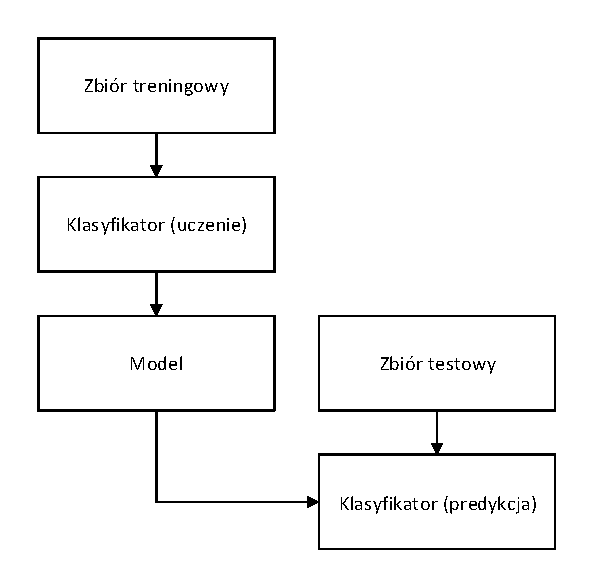
\includegraphics{diagrams/uczenie-predykcja.pdf}
	\caption{Wykorzystanie danych w~modelu predykcji}
\end{figure}


%%%%%%%%%%%%%%%%%%%%%%%%%%%%%%%%%%%%%%%%%%%%%%%%%%%%%%%%%%%%
%%%%%%%%%%%%%%%%%%%%%%%%%%%%%%%%%%%%%%%%%%%%%%%%%%%%%%%%%%%%
\section{Rola metryk w~in�ynierii oprogramowania}
\label{rola-metryk}

\noindent Norma IEEE 1061-1998 \cite{749159} definiuje metryk� jako ``funkcj� odwzorowuj�c� jednostk� oprogramowania w~warto�� liczbow�. Ta wyliczona warto�� jest interpretowalna jako stopie� spe�nienia pewnej w�asno�ci jako�ci jednostki oprogramowania."

W in�ynierii oprogramowania metryki s� wykorzystywane we wszystkich fazach procesu wytwarzania oprogramowania. Pozwalaj� na por�wnywanie ze sob� r�nych element�w lub r�nych projekt�w poniewa� s� danymi liczbowymi. W~fazie projektowania mog� s�u�y� m.in. do szacowania nak�adu pracy potrzebnego do realizacji projektu. W~fazie produkcji i~test�w do mierzenia jako�ci aplikacji, wydajno�ci pracy czy z�o�ono�ci programu.

Metryki mo�na podzieli� wed�ug r�nych kryeri�w. Ze wzgl�du na typ artefaktu jaki opisuj� dzieli si� je na:
\begin{itemize}
	\item Metryki produktu (inaczej metryki kodu �r�d�owego). S� bezpo�rednio wyliczane z~kodu �r�d�owego programu. Przyk�adem takich metryk s�:
	\begin{itemize}
		\item Zestaw metryk CK \cite{chidamber1994metrics}, do kt�rego nale��:
		\begin{itemize}
			\item u�rednione metody na klas� (ang. \textit{Weighted Methods per Class}, WMC),
			\item g��boko�� drzewa dziedziczenia (ang. \textit{Depth of Inheritance Tree}, DIT),
			\item liczba dzieci (ang. \textit{Number of Children}, NOC),
			\item zale�no�� mi�dzy obiektami (ang. \textit{Coupling Between Objects}, CBO),
			\item odpowiedzialno�� danej klasy (ang. \textit{Response For a~Class}, RFC),
			\item brak sp�jno�ci metod (ang. \textit{Lack of Cohesion of Methods}, LCOM).
		\end{itemize}
		\item OO --- metryki obiektowe, np.:
		\begin{itemize}
			\item liczba atrybut�w (ang. \textit{Number of attributes}, NOA),
			\item liczba metod (ang. \textit{Number of methods}, NOM),
			\item liczba dziedziczonych metod (ang. \textit{Number of methods inherited}, NOMI).
		\end{itemize}
		\item LOC --- liczba linii kodu.
	\end{itemize}
	\item Metryki procesu (inaczej metryki zmian) \cite{madeyski2014process}. Okre�laj� zmienno�� atrybutu w~czasie. Oblicza si� je dla zadanych przedzia��w czasowych. Niezb�dna do ich obliczenia jest historia projektu, kt�r� mo�na uzyska� dzi�ki systemom kontroli wersji (jak SVN czy Git). Przyk�ady metryk procesu:
		\begin{itemize}
			\item liczba modyfikacji (rewizji) pliku (ang. \textit{Number of Revisions}, NR),
			\item liczba autor�w zmieniaj�cych plik (ang. \textit{Number of Distinct Commiters}, NDC),
			\item liczba zmienionych linii kodu (ang. \textit{Number of Modified Lines}, NML),
			\item wiek pliku (ang. \textit{Age}, AGE),
			\item liczba refaktoryzacji pliku (ang. \textit{(Number of Refactorings}, NREF),
			\item liczba dodanych (usuni�tych, zmienionych) metod,
			\item liczba dodanych (usuni�tych, zmienionych) atrybut�w.
		\end{itemize}
\end{itemize}

Dodatkowo mo�na podzieli� metryki z~uwagi na cel pomiaru \cite{gorski2000inzynieria}:
\begin{itemize}
	\item metryki z�o�ono�ci,
	\item metryki szacowania nak�adu,
	\item metryki funkcjonalno�ci.
\end{itemize}


Model predykcji defekt�w to narz�dzie, kt�re na podstawie warto�ci metryk danego projektu dokonuje wskazania defekt�w znajduj�cych si� w~tym projekcie. Aby poprawnie zinterpretowa� wskazania dostarczane przez model predykcji defekt�w nale�y okre�li� czym jest defekt. Norma 982.2 IEEE/ANSI \cite{26479} definiuje defekt jako anomali� w~produkcie, kt�ra mo�e by�:
\begin{itemize}
	\item zaniechaniami i~niedoskona�o�ciami znalezionymi podczas wczesnych faz cyklu �ycia oraz
	\item b��dami zawartymi w~oprogramowaniu wystarczaj�co dojrza�ym do testowania lub dzia�ania.
\end{itemize}

Istniej�ce badania wykaza�y, �e metryki procesu przewy�szy�y metryki produktu w~kontek�cie budowania modeli predykcji defekt�w \cite{giger2012method, kamei2010revisiting, mende2009revisiting, ferzund2009empirical}. Z~tego powodu w~dalszej cz�ci pracy zrezygnowano z~wykorzystania metryk produktu, bior�c pod uwag� jedynie metryki procesu.






%%%%%%%%%%%%%%%%%%%%%%%%%%%%%%%%%%%%%%%%%%%%%%%%%%%%%%%%%%%%
%%%%%%%%%%%%%%%%%%%%%%%%%%%%%%%%%%%%%%%%%%%%%%%%%%%%%%%%%%%%
\section{Koszty zapewnienia jako�ci}

\noindent W~in�ynierii oprogramowania wyst�puje kilka r�nych definicji jako�ci. Na potrzeby niniejszej pracy przyj�to definicj� Kana \cite{kan2002metrics} ``brak defekt�w w~produkcie". Zarz�dzanie jako�ci� oprogramowania polega na podejmowaniu dzia�a� maj�cych na celu zapewnienie jako�ci tworzonego oprogramowania poprzez szereg test�w, kt�re wspieraj� ca�y proces rozwoju oprogramowania.
\begin{itemize}
	\item Na etapie zbierania wymaga� --- weryfikacja czy okre�lone wymagania b�d� mo�liwe do zweryfikowania (przetestowania).
	\item Na etapie projektowania --- zaplanowanie procesu testowego, wyb�r �rodowisk testowych.
	\item Na etapie kodowania --- definiowanie i~realizacja scenariuszy i~przypadk�w testowych oraz rejestracja defekt�w.
	\item Na etapie zamkni�cia projektu --- testy integracyjne, testy akceptacyjne, testy operacyjne.
\end{itemize}

\noindent Jak wykaza� Arisholm i~in. w~\cite{arisholm2010systematic} koszty zapewnienia jako�ci s� prawie proporcjonalne do wielko�ci modu�u. Dlatego badacze bior� pod uwag� wysi�ek zwi�zany z~dzia�aniami maj�cymi na celu zapewnienie jako�ci \cite{rahman2011bugcache, koru2008theory, menzies2010defect}. Zmniejszenie wysi�ku i~kosztu zwi�zanego z~zapewnieniem jako�ci to obecnie jeden z~g��wnych kierunk�w bada� \cite{hata2012bug}.

Podstawowym celem pracy dyplomowej jest stworzenie narz�dzi w~postaci wtyczek do �rodowiska KNIME, s�u��cych do gromadzenia metryk oprogramowania z~system�w kontroli wersji oraz zgromadzenie jak najwi�kszej ilo�ci metryk w~publicznym repozytorium. Nast�pnym krokiem jest stworzenie modelu (modeli) predykcji defekt�w oraz ich ewaluacja, bior�c pod uwag� wysi�ek zwi�zany z~zapewnieniem jako�ci oprogramowania. Stworzenie narz�dzi pozwalaj�cych na zautomatyzowane gromadzenie metryk z~dost�pnych projekt�w (na przyk�ad open source) pozwoli rozszerzy� publiczne zbiory danych. Dzi�ki temu b�dzie mo�liwe wykorzystanie tych danych do tworzenia modeli predykcji defekt�w oprogramowania dzi�ki: wi�kszym zbiorom ucz�cym; ewaluacji modeli na wi�kszych zbiorach danych.







%%%%%%%%%%%%%%%%%%%%%%%%%%%%%%%%%%%%%%%%%%%%%%%%%%%%%%%%%%%%
%%%%%%%%%%%%%%%%%%%%%%%%%%%%%%%%%%%%%%%%%%%%%%%%%%%%%%%%%%%%
\section{Systemy kontroli wersji jako �r�d�o danych o~projektach}

\noindent Jak wspomniano wcze�niej w~rozdziale \ref{rola-metryk} aby obliczy� metryki procesu, konieczne jest uzyskanie historii projektu. Przegl�d literatury pozwoli� na wyodr�bnienie sposob�w i~narz�dzi, kt�re pozwalaj� na por�wnywanie r�nych wersji kodu �r�d�owego. Jak wykaza� Kamei i~in. w~\cite{kamei2010revisiting, posnett2011ecological, nguyen2010studying} predykcja na poziomie plik�w jest bardziej efektywna ni� na poziomie pakiet�w. Id�c dalej w~kierunku uszczeg�owienia wynik�w predykcji, mo�na przypuszcza�, �e predykcja na poziomie metod by�aby skuteczniejsza ni� na poziomie plik�w. Badanie \cite{hata2012bug} wykaza�o, �e pliki zawieraj�ce b��dy zawieraj� prawie lub ponad 10 metod, natomiast tylko kilka metod zawiera b��dy (mediana 1--2). Jest to nie tylko odpowied� na pytanie czy predykcja na poziomie metod jest skuteczniejsza, ale r�wnie� wskazanie przyczyny takiego stanu rzeczy. Jednak�e aby w~pe�ni wykorzysta� mo�liwo�ci ograniczenia koszt�w jako�ci poprzez predykcj� na poziomie metod, potrzebne s� skuteczne modele, dostarczaj�ce wiarygodnych wynik�w.

Ze wzgl�du na powy�sze zale�no�ci, podj�to decyzj� o~prowadzeniu dalszych prac w~kierunku budowy modeli predykcji na poziomie metod. Poni�ej wypisano techniki por�wnywania kodu �r�d�owego na poziomie metod.
\begin{itemize}
	\item ChangeDistiller \cite{fluri2007change} --- polega na odwzorowaniu kodu �r�d�owego Java w~strukturze drzewiastej, jak� jest AST (ang. \textit{Abstract Syntax Tree}) a~nast�pnie wyodr�bnieniu zmian pomi�dzy dwiema wersjami przy u�yciu algorytm�w por�wnywania drzew.
	\item Historage \cite{hata2011historage} --- wykorzystuje system kontroli wersji Git do przechowywania zidentyfikowanych zmian w~kodzie na niskim poziomie.
	\item APFEL \cite{zimmermann2006fine} --- jest wtyczk� do �rodowiska Eclipse, kt�ra zbiera w~bazie danych niskopoziomowe zmiany w~kodzie. Dzia�a z~systemem kontroli wersji CVS i~�r�d�ami Java.
	\item C-REX \cite{hassan2004c} --- wyodr�bnia fakty z~historii kodu �r�d�owego j�zyka C, a~nast�pnie por�wnuje ze sob� kolejne wersje.
	\item Kenyon \cite{bevan2005facilitating}.
	\item Beagle \cite{godfrey2005using}.
\end{itemize}






%%%%%%%%%%%%%%%%%%%%%%%%%%%%%%%%%%%%%%%%%%%%%%%%%%%%%%%%%%%%
\subsection{Historia b��d�w w~projektach}
\label{linkowanie-bledow}

\noindent Metryki, kt�re stanowi� dane wej�ciowe w~modelach predykcji s� zmiennymi niezale�nymi (ang. \textit{independent variables}). Pe�ny zestaw danych potrzebny do wytrenowania modelu obejmuje tak�e zmienne zale�ne (ang. \textit{dependent variables}). Zmienna niezale�na reprezentuje wyj�cie (wynik), oraz mo�e by� u�ywana do testowania modelu, �eby oceni� jego skuteczno��. W~predykcji defekt�w oprogramowania zmienn� zale�n� jest liczba b��d�w lub zmienna okre�laj�ca czy wyst�puje b��d.

Aby uzyska� informacje o~b��dach w~projekcie stosuje si� metody linkowania b��d�w. Linkowanie polega na odszukaniu powi�za� pomi�dzy zmian� zapisan� w~repozytorium kodu, a~b��dem zg�oszonym w~systemie �ledzenia zmian (ang. \textit{Issue Tracking System}, ITS), takim jak JIRA, Bugzilla, IBM Rational ClearQuest czy innym.

Metoda u�ywana w~tej pracy opiera si� na metodzie SZZ \cite{sliwerski2005changes}. Jej podstawow� zalet� jest por�wnywanie czasu naprawienia b��du zapisanego w~ITS z~czasem wys�ania poprawki do systemu kontroli wersji. Dzi�ki takiemu por�wnaniu wyklucza si� du�� liczb� b��dnych wskaza�, kt�re wynikaj� z~niew�a�ciwego lub przypadkowego przyporz�dkowania b��du do zmiany kodu. Przyczyn� takich b��dnych dopasowa� mo�e by� umieszczenie w~opisie zmiany ci�gu numerycznego nieb�d�cego numerem b��du.






%%%%%%%%%%%%%%%%%%%%%%%%%%%%%%%%%%%%%%%%%%%%%%%%%%%%%%%%%%%%
\chapter{Om�wienie infrastruktury pomiarowej}
\label{rozdzial3}
\noindent
Badania zgodnie z~za�o�eniami przeprowadzono w~�rodowisku KNIME rozszerzonym o~wtyczki z~DePress. Dodatkowo w~KNIME u�yto algorytm�w klasyfikacji z~pakietu Weka.

%%%%%%%%%%%%%%%%%%%%%%%%%%%%%%%%%%%%%%%%%%%%%%%%%%%%%%%%%%%%
%%%%%%%%%%%%%%%%%%%%%%%%%%%%%%%%%%%%%%%%%%%%%%%%%%%%%%%%%%%%
\section{KNIME}

\noindent KNIME jest platform� do analizy danych, kt�ra umo�liwia wykonywanie zaawansowanych statystyk i~eksploracji danych, w~celu analizy trend�w i~przewidywania wynik�w. Wizualny zestaw narz�dzi pozwala na pozyskiwani danych, przekszta�canie ich, wst�pne rozpoznanie, analizy predykcyjne i~wizualizacj�. KNIME daje r�wnie� mo�liwo�� tworzenia raport�w na podstawie zgromadzonych informacji. KNIME Desktop jest oprogramowaniem o~otwartym kodzie (ang. \textit{open source}) udost�pnianym na licencji GPL \cite{BCDG+07}.

\begin{figure}[htbp]
	\centering
	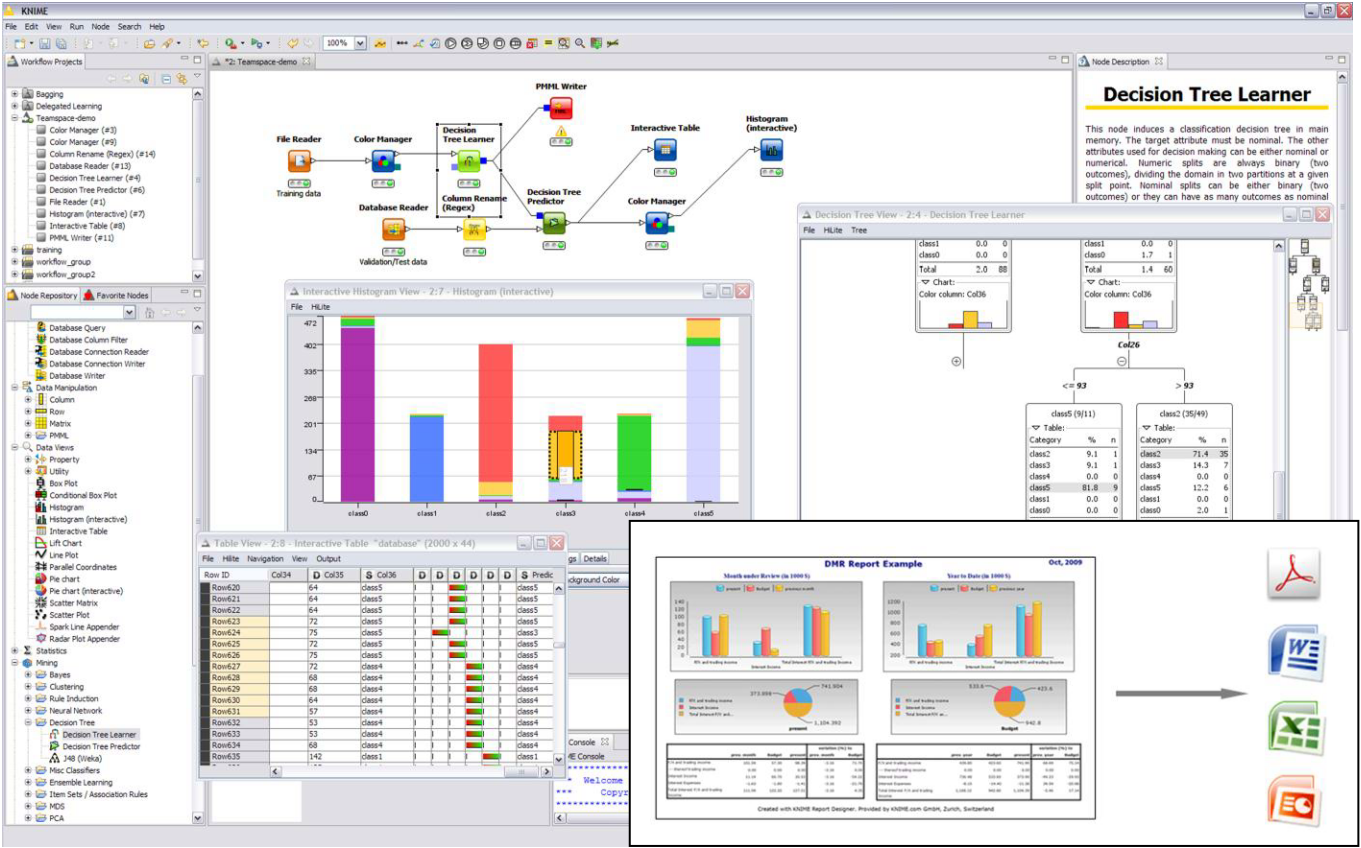
\includegraphics[width=1\textwidth]{img/knime-gui}
	\caption{Interejs KNIME. �r�d�o \cite{BCDG+07}}
\end{figure}

Platforma KNIME zawiera setki w�z��w pozyskiwania danych, przetwarzania i~filtrowania, analizy i~eksploracji danych, wizualizacji i~innych. Oprogramowanie bazuje na platformie Eclipse\footnote{http://eclipse.org} i~jest rozszerzalne poprzez system wtyczek, dzi�ki czemu znajduje zastosowanie w~komercyjnych �rodowiskach produkcyjnych jak i~�rodowiskach badawczych. Przyk�ad procesu analizy i~eksploracji danych przedstawiono na rysunku \ref{knime-workflow}.

\begin{figure}[htbp]
	\centering
	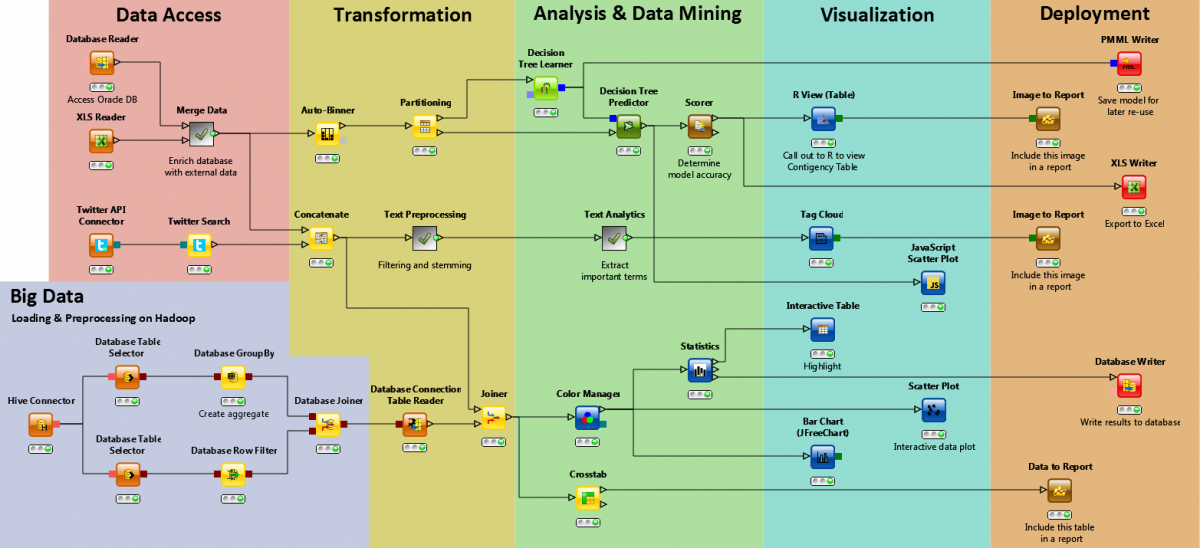
\includegraphics[width=1\textwidth]{img/knime-workflow}
	\caption{Proces zbudowany w~KNIME. �r�d�o \cite{BCDG+07}}
	\label{knime-workflow}
\end{figure}

\paragraph{Budowanie procesu.} Proces jest tworzony z~w�z��w dost�pnych w~programie. W�z�y umieszcza si� w~edytorze i~��czy ze sob�. S� one podstawowymi jednostkami w~procesie. Ka�dy w�ze� mo�e mie� porty wej�ciowe i~wyj�ciowe. Dane s� przekazywane pomi�dzy w�z�ami z~portu wyj�ciowego jednego w�z�a do portu wej�ciowego innego w�z�a. Wyj�cie w�z�a mog� stanowi� na przyk�ad dane tabelaryczne, obraz, model zapisany w~PMML (ang. \textit{Predictive Model Markup Language}) i~inne.

\begin{figure}[htbp]
	\centering
	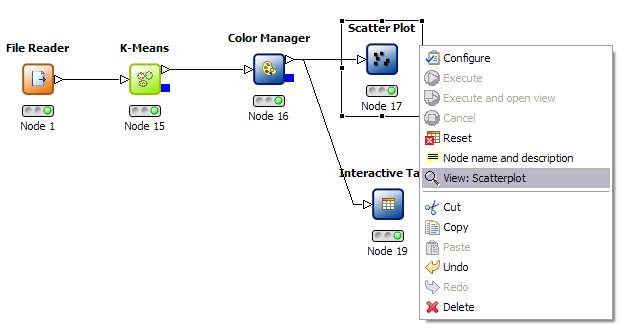
\includegraphics[width=1\textwidth]{img/knime-connected-nodes}
	\caption{W�z�y KNIME. �r�d�o \cite{BCDG+07}}
\end{figure}

W�ze� przed u�yciem musi zosta� skonfigurowany. Ka�dy rodzaj w�z�a posiada sw�j zestaw parametr�w konfigurowalnych za pomoc� interfejsu graficznego. Prawid�owo skonfigurowany w�ze� mo�e utowrzy� na wyj�ciu tabel� danych, k�tra mo�e by� ogl�dana w~wewn�trznym edytorze. Opr�cz tabeli danych niekt�re w�z�y udost�pniaj� widoki. Widokiem mo�e by� np. wykres, graf, tabela, itd. Widoki mog� zawiera� elementy interaktywne pozwalaj�ce na dostosowywanie prezentowanych danych, zmian� uk�adu, kolor�w, typu wykresu, itp.



%%%%%%%%%%%%%%%%%%%%%%%%%%%%%%%%%%%%%%%%%%%%%%%%%%%%%%%%%%%%
%%%%%%%%%%%%%%%%%%%%%%%%%%%%%%%%%%%%%%%%%%%%%%%%%%%%%%%%%%%%
\section{R}

\noindent R~jest darmowym �rodowiskiem i~j�zykiem do oblicze� statystycznych i~wizualizacji. Jest podobny do j�zyka i~�rodowiska S. Ma szerokie zastosowanie na �wiecie, jest podstawowym narz�dziem w~bioinformatyce, u�ywa si� go w~takich firmach jak Facebook, Google, Form, Mozilla czy Twitter. Wiele pakiet�w statystycznych (np. RapidMiner, KNIME) oferuje mechanizmy zapewniaj�ce wsp�prac� z~R.

R jest zbudowany w~architekturze modu�owej. Jest rozszerzalny za pomoc� pakiet�w zawieraj�cych dodatkowe funkcje lub dodatkowe narz�dzia przeznaczone dla poszczeg�lnych dziedzin nauki. Zalet� R~jest tak�e mo�liwo�� tworzenia wysokiej jako�ci grafik gotowych do publikacji. Tworzenie grafik jest uproszczone poprzez stosowanie gotowych szablon�w, z~jednoczesnym zachowaniem mo�liwo�ci pe�nej kontroli i~personalizacji przez u�ytkownika. Ma tak�e sw�j w�asny format dokumentacji podobny do LaTeX.




%%%%%%%%%%%%%%%%%%%%%%%%%%%%%%%%%%%%%%%%%%%%%%%%%%%%%%%%%%%%
%%%%%%%%%%%%%%%%%%%%%%%%%%%%%%%%%%%%%%%%%%%%%%%%%%%%%%%%%%%%
\section{DePress}
\label{depress}

\noindent DePress jest oparty wy��cznie na architekturze wtyczek KNIME, dzi�ki czemu mo�liwa jest integracja i~wsp�dzia�anie z~istniej�cymi wtyczkami. G��wnym zadaniem pakietu jest predykcja defekt�w oprogramowania. Poszczeg�lne wtyczki dostarczaj� odpowiednich funkcji w~zale�no�ci od ich przeznaczenia. Podzielono je na trzy g��wne grupy (rysunek \ref{depress-struktura}):
\begin{itemize}
	\item Adaptery --- pozwalaj� na pobieranie danych z~zewn�trznych narz�dzi.
	\item Generatory metryk --- wyliczaj� metryki na podstawie danych wej�ciowych.
	\item Inne --- dostarczaj� metod do dodatkowych przekszta�ce� danych.
\end{itemize}

\begin{figure}[htbp]
	\centering
	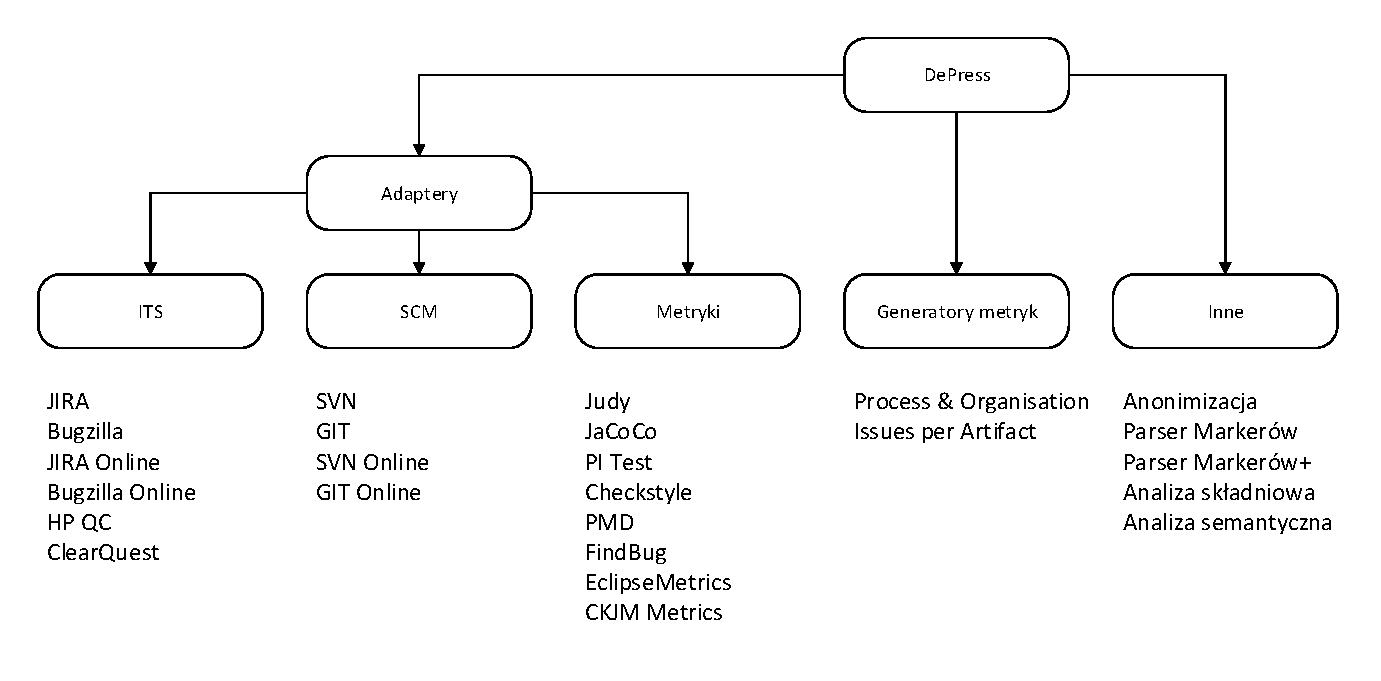
\includegraphics[width=1\textwidth]{diagrams/depress.pdf}
	\caption{Struktura DePress. �r�d�o \cite{madeyski2014software}}
	\label{depress-struktura}
\end{figure}

Dzi�ki separacji wtyczek jest mo�liwa �atwa zamiana jednej wtyczki na inn�. Na przyk�ad gdy analizuj�c projekt oka�e si�, �e zosta� on przeniesiony z~SVN do Git, wystarczy u�y� odpowiedniej wtyczki adaptera aby na nowo pobra� dane o~projekcie.

W badaniu u�yto wtyczek adapter�w Jira (Online) i~Bugzilla (Online) do pobierania danych o~zg�oszonych b��dach z~system�w �ledzenia zagadnie� (ang. \textit{Issue Tracking System}, ITS). Istniej�ce wtyczki adapter�w do wsp�pracy z~systemami kontroli wersji (SCM) okaza�y si� nie wystarczaj�ce, poniewa� dostarczaj� tylko danych o~zmianach na poziomie klas. Potrzebne by�o stworzenie nowej wtyczki AstMetrics do ekstrakcji zmian na niskim poziomie granulacji.


%%%%%%%%%%%%%%%%%%%%%%%%%%%%%%%%%%%%%%%%%%%%%%%%%%%%%%%%%%%%
%%%%%%%%%%%%%%%%%%%%%%%%%%%%%%%%%%%%%%%%%%%%%%%%%%%%%%%%%%%%
\section{AstMetrics}
\label{metryki}

\noindent Wtyczka AstMetrics w~pierwszej wersji zosta�a napisana przez Piotra Mitk� \cite{mitka}. Na potrzeby tego badania zosta�a w~du�ej cz�ci napisana od nowa i~poszerzona o~nowe metryki. Bazuj�c na oprogramowaniu Change Distiller \cite{fluri2007change} dokonuje ona por�wnania historycznych wersji kodu �r�d�owego ka�dego pliku pobranego z~repozytorium. Ka�da wersja pliku jest odwzorowywana za pomoc� drzewa AST (ang. \textit{Abstract Syntax Tree}) a~nast�pnie drzewa s� por�wnywane pomi�dzy kolejnymi wersjami (patrz rysunek \ref{ast-compare}). Na tej podstawie jest mo�liwe wykrycie zmian w~kodzie �r�d�owym na niskim poziomie granulacji. Zmiany s� zapisywane w~tymczasowej bazie danych a~nast�pnie s� wyliczane z~nich metryki dla ka�dej metody z~ka�dej klasy znajduj�cej si� w~kodzie �r�d�owym.

\begin{figure}[htbp]
	\centering
	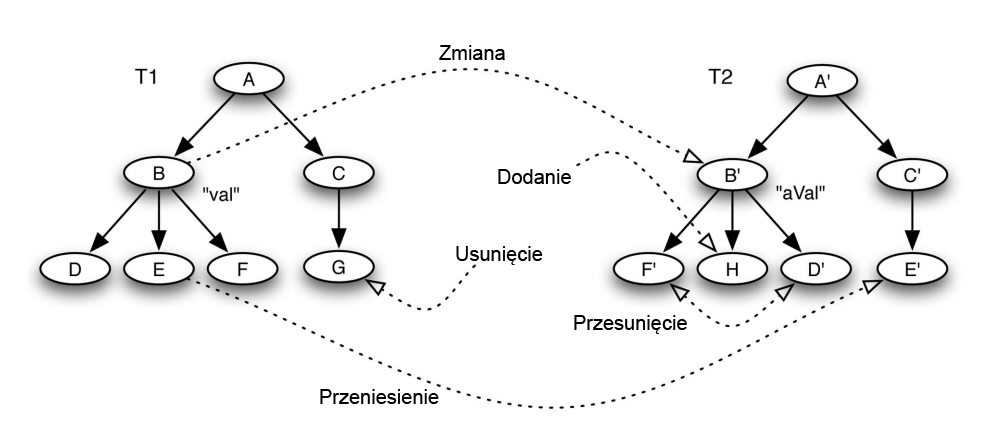
\includegraphics[width=1\textwidth]{img/ast-compare}
	\caption{Por�wnanie drzewa AST. �r�d�o \cite{fluri2007change}}
	\label{ast-compare}
\end{figure}

Metryki wyliczane w~pierwszej wersji wtyczki zosta�y zawarte w~tabeli \ref{metryki1} a~dodane w~drugiej wersji wtyczki w~tabeli \ref{metryki2}.


\begin{table}[htbp]
	\caption{Metryki wyliczane w~pierwszej wersji wtyczki AstMetrics}
	\label{metryki1}
	\begin{center}
		\begin{tabular}{@{}ll@{}}
			\toprule
			\bf Nazwa metryki &
			\bf Opis \\
			\midrule
			allMethodHistories & ile razy metoda by�a zmieniana w~historii                   \\
			methodHistories    & ile razy metoda by�a zmieniana w~danych przedziale czasowym \\
			authors            & liczba autor�w                                              \\
			stmtAdded          & ��czna liczba dodanych instrukcji                           \\
			maxStmtAdded       & maksymalna liczba dodanych instrukcji                       \\
			avgStmtAdded       & �rednia liczba dodanych instrukcji                          \\
			stmtUpdated        & ��czna liczba zmienionych instrukcji                        \\
			maxsSmtUpdated     & maksymalna liczba zmienionych instrukcji                    \\
			avgStmtUpdated     & �rednia liczba zmienionych instrukcji                       \\
			stmtDeleted        & ��czna liczba usuni�tych instrukcji                         \\
			maxStmtDeleted     & maksymalna liczba usuni�tych instrukcji                     \\
			avgStmtDeleted     & �rednia liczba usuni�tych instrukcji                        \\
			stmtParentChanged  & ��czna liczba zmienionych instrukcji nadrz�dnych            \\
			churn              & suma stmtAdded i~stmtDeleted we wszystkich wersjach         \\
			maxChurn           & maksymalna warto�� churn na przestrzeni wersji              \\
			avgChurn           & �rednia warto�� churn na przestrzeni wersji                 \\
			decl               & ��czna liczba zmian deklaracji metody                       \\
			cond               & ��czna liczba zmian deklaracji warunkowych                  \\
			elseAdded          & ��czna liczba dodanych cz�ci \textit{else}                 \\
			elseDeleted        & ��czna liczba usuni�tych cz�ci \textit{else}               \\
			\bottomrule
		\end{tabular}
	\end{center}
\end{table}

\begin{table}[htbp]
	\caption{Metryki dodane w~drugiej wersji wtyczki AstMetrics}
	\label{metryki2}
	\begin{center}
		\begin{tabular}{@{}ll@{}}
			\toprule
			\bf Nazwa metryki &
			\bf Opis \\
			\midrule
			loopsAdded & ��czna liczba dodanych p�tli \\
			loopsUpdated & ��czna liczba zmienionych p�tli \\
			loopsDeleted & ��czna liczba usuni�tych p�tli \\
			variablesAdded & ��czna liczba dodanych instrukcji deklaracji zmiennej \\
			variablesUpdated & ��czna liczba zmienionych instrukcji deklaracji zmiennej \\
			variablesDeleted & ��czna liczba usuni�tych instrukcji deklaracji zmiennej \\
			assigmentsAdded & ��czna liczba dodanych instrukcji przypisania \\
			assigmentsUpdated & ��czna liczba zmienionych instrukcji przypisania \\
			assigmentsDeleted & ��czna liczba usuni�tych instrukcji przypisania \\
			returnsAdded & ��czna liczba dodanych instrukcji \textit{return} \\
			returnsUpdated & ��czna liczba zmienionych instrukcji \textit{return} \\
			returnsDeleted & ��czna liczba usuni�tych instrukcji \textit{return} \\
			nullsAdded & ��czna liczba dodanych instrukcji zawieraj�cych \textit{null} \\
			nullsUpdated & ��czna liczba zmienionych instrukcji zawieraj�cych \textit{null} \\
			nullsDeleted & ��czna liczba usuni�tych instrukcji zawieraj�cych \textit{null} \\
			casesAdded & ��czna liczba dodanych instrukcji warunkowych \textit{case} \\
			casesUpdated & ��czna liczba zmienionych instrukcji warunkowych \textit{case} \\
			casesDeleted & ��czna liczba usuni�tych instrukcji warunkowych \textit{case} \\
			breaksAdded & ��czna liczba dodanych instrukcji \textit{break} \\
			breaksUpdated & ��czna liczba zmienionych instrukcji \textit{break} \\
			breaksDeleted & ��czna liczba usuni�tych instrukcji \textit{break} \\
			objectsAdded & ��czna liczba dodanych instrukcji tworz�cych obiekt \\
			objectsUpdated & ��czna liczba zmienionych instrukcji tworz�cych obiekt \\
			objectsDeleted & ��czna liczba usuni�tych instrukcji tworz�cych obiekt \\
			catchesAdded & ��czna liczba dodanych blok�w przechwytywania wyj�tku \\
			catchesUpdated & ��czna liczba zmienionych blok�w przechwytywania wyj�tku \\
			catchesDeleted & ��czna liczba usuni�tych blok�w przechwytywania wyj�tku \\
			throwsAdded & ��czna liczba dodanych blok�w rzucania wyj�tku \\
			throwsUpdated & ��czna liczba zmienionych blok�w rzucania wyj�tku \\
			throwsDeleted & ��czna liczba usuni�tych blok�w rzucania wyj�tku \\
			\bottomrule
		\end{tabular}
	\end{center}
\end{table}

Dodatkowo zaimplementowano drugie wyj�cie wtyczki z~wszystkimi historiami metod, tj. z~informacjami o~tym kt�ra metoda zosta�a zmieniona w~danej wersji historycznej w~repozytorium kodu. W~zwi�zku z~tym, �e do repozytorium s� zapisywane zmiany w~pojedycznych plikach, a~nie bardziej szczeg�owe, wyst�pi�a potrzeba stworzenia takiego zestawienia. Struktura tworzonej tabeli danych zosta�a przedstawiona w~tabeli \ref{ast-histories}. Dane historyczne s�u�� do wyszukiwania defekt�w w~kodzie �r�d�owym, kt�re zosta�o opisane w~rozdziale \ref{wyszukiwanie-defektow}.

\begin{table}[htbp]
	\caption{Struktura tabeli wyj�ciowej z~danymi historycznymi wtyczki AstMetrics}
	\label{ast-histories}
	\begin{center}
		\begin{tabular}{@{}ll@{}}
			\toprule
			\bf Nazwa kolumny &
			\bf Opis \\
			\midrule
			MethodName & Nazwa metody                  \\
			Author     & Autor zmiany                  \\
			Message    & Opis zmiany                   \\
			Date       & Data przes�ania               \\
			CommitID   & Unikalny identyfikator zmiany \\
			\bottomrule
		\end{tabular}
	\end{center}
\end{table}

Do prawid�owego dzia�ania wtyczki wymagane jest okre�lenie warto�ci parametr�w:
\begin{itemize}
	\item dirname - katalog ze sklonowanym repozytorium git (np. \textit{C:/ant} lub \textit{/home/user/ant},
	\item package - pakiet, kt�ry zostanie uwzgl�dniony w~tabelach wyj�ciowych (np. \textit{org.apache.ant}),
	\item exclude\_dir - katalog, kt�ry zostanie wy��czony z~pobieranai danych (np. \textit{src/tests}),
	\item bottom\_commit - identyfikator rewizji pocz�tkowej, dozwolone jest podanie identyfikatora SHA-1, tagu poprzedzonego napisem \textit{tag:} lub napis \textit{initial} oznaczaj�cego pierwsz� (najstarsz�) rewizj� w~repozytorium,
	\item top\_commit - identyfikator rewizji ko�cowej, czyli rewizji dla kt�rej zostan� obliczone metryki, dozwolone jest podanie identyfikatora SHA-1 lub tagu poprzedzonego napisem \textit{tag:},
	\item top\_commit\_post\_rel - identyfikator rewizji zamykaj�cej, pomi�dzy t� wersj� a~wersj� \textit{top\_commit} zostanie pobrana historia repozytorium, dozwolone jest podanie identyfikatora SHA-1, tagu poprzedzonego napisem \textit{tag:} lub napis \textit{current} oznaczaj�cego ostatni� (najnowsz�) rewizj� w~repozytorium.
\end{itemize}

Dzia�anie wtyczki obrazuje rysunek \ref{ast-metrics-process}.


\begin{figure}[htbp]
	\centering
	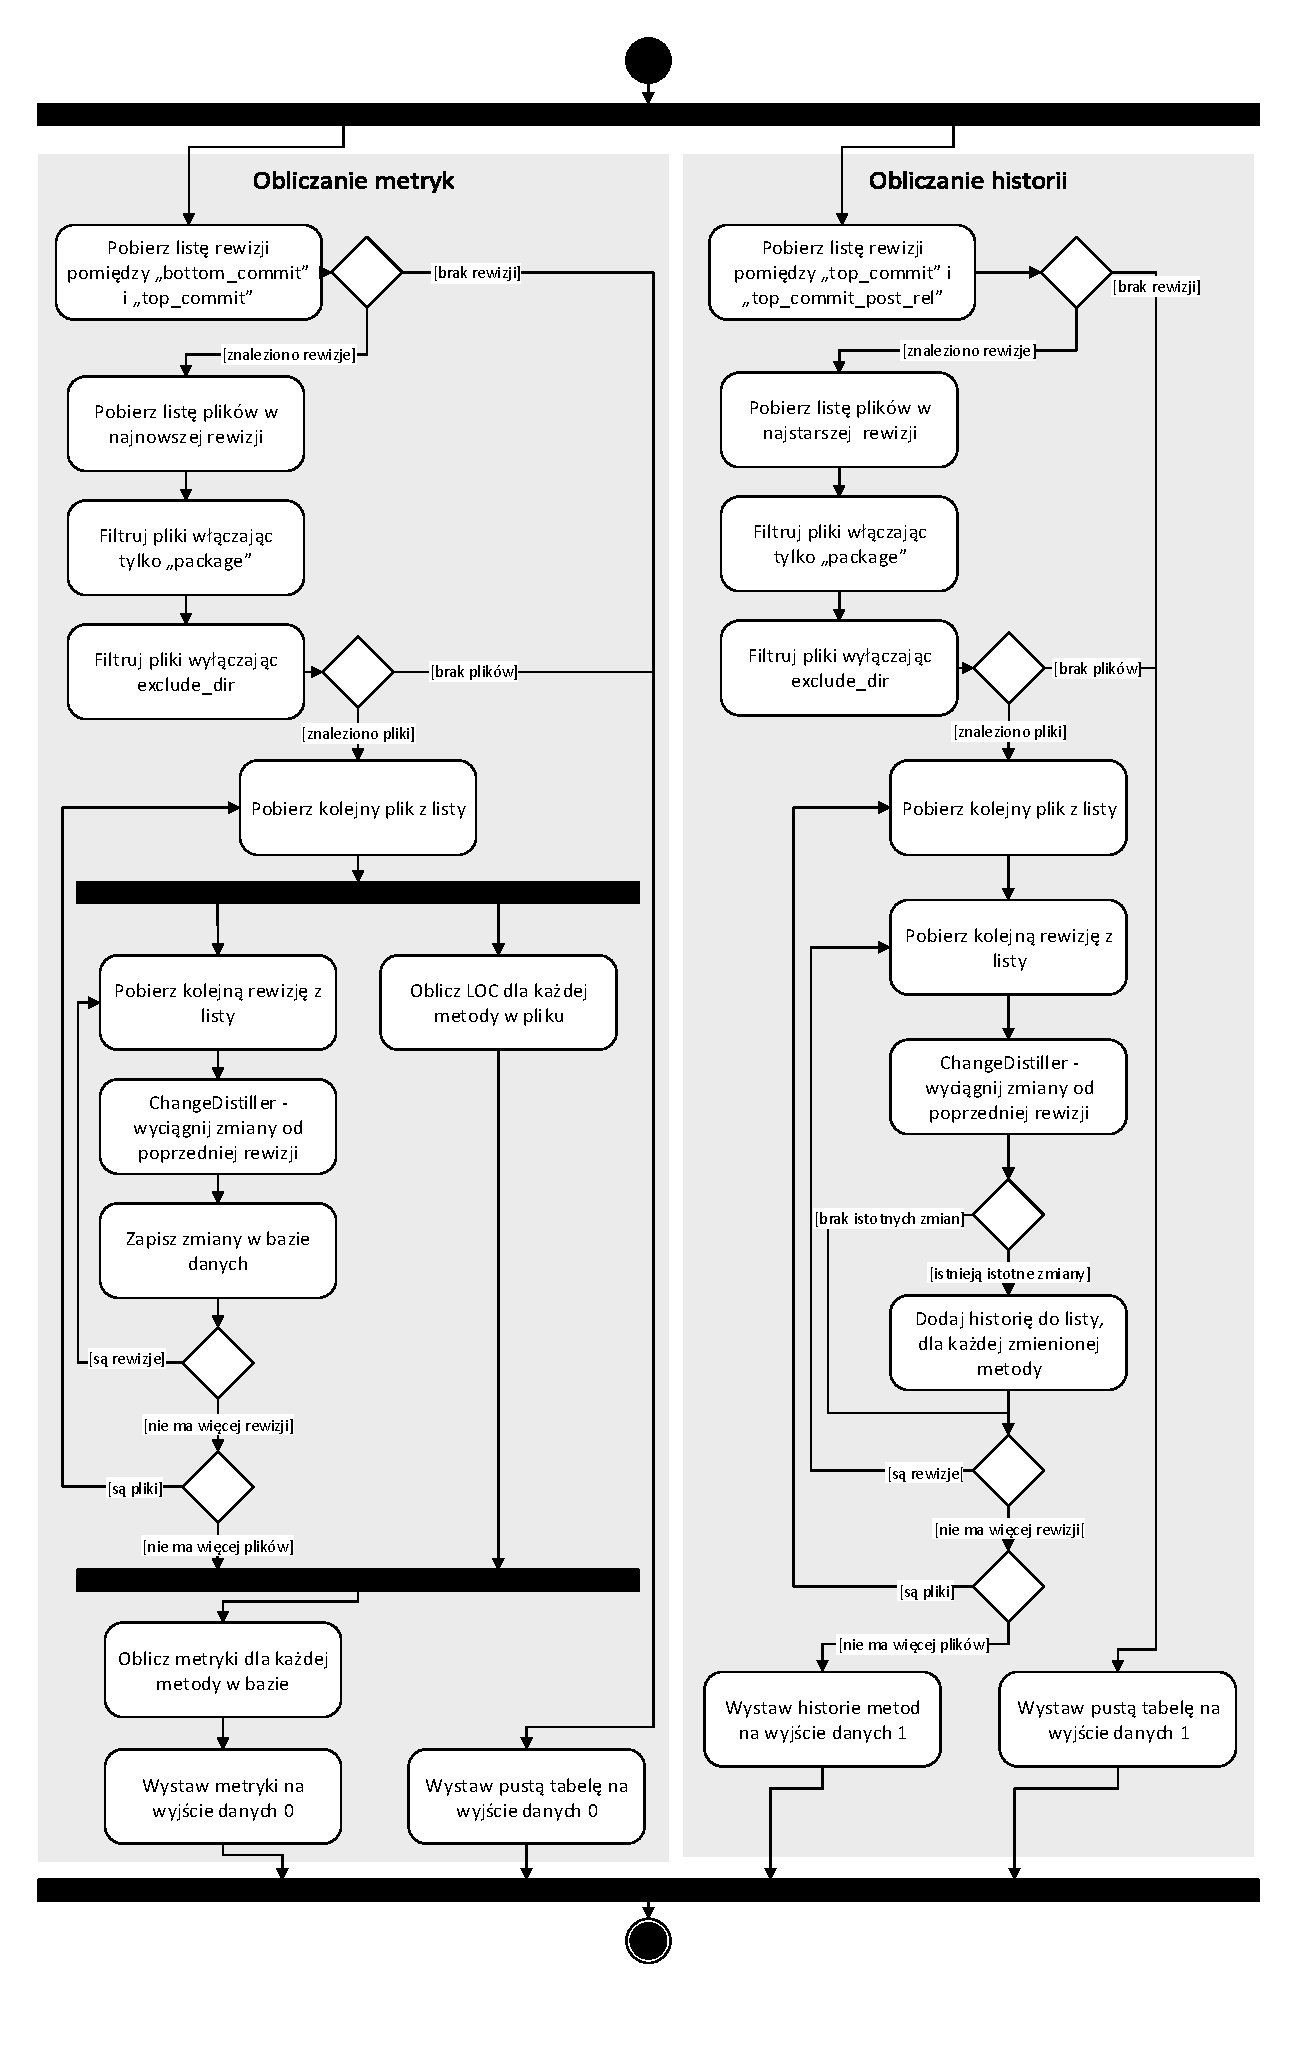
\includegraphics[width=1\textwidth]{diagrams/ast-metrics-process.pdf}
	\caption{Diagram aktywno�ci wtyczki AstMetrics}
	\label{ast-metrics-process}
\end{figure}



%%%%%%%%%%%%%%%%%%%%%%%%%%%%%%%%%%%%%%%%%%%%%%%%%%%%%%%%%%%%
\subsection{Gromadzenie metryk}

\noindent Do trenowania i~oceny algorytm�w klasyfikacji cz�sto stosuje si� walidacj� krzy�ow�, polegaj�c� na podziale zbioru danych na dwa podzbiory --- treningowy i~testowy --- a~nast�pnie wykorzystaniu ich zgodnie z~przeznaczeniem. W~niniejszej pracy zastosowano inne podej�cie, polegaj�ce na wykorzystaniu dw�ch niezale�nych zbior�w danych z~dw�ch r�nych wyda� oprogramowania. Metryki wersji A~pos�u�y�y jako zbi�r treningowy a~metryki wersji B~jako zbi�r testowy. Zalet� takiego podej�cia jest lepsze dopasowanie do rzeczywistych warunk�w wyst�puj�cych w~procesie wytwarzania oprogramowania. W~tabeli \ref{wersje} zawarto informacje o~przebadanym oprogramowaniu wraz z~oznaczeniami wersji A~i~B. Metryki zosta�y wyliczone z~u�yciem wtyczki AstMetrics. Wprowadzono r�wnie� dodatkowo� metryk� pomocnicz� LOC (ang. \textit{ang. Lines of code}) - liczba linii kodu.

\begin{table}[htbp]
	\small
	\caption{Przegl�d projekt�w wykorzystanych do badania}
	\label{wersje}
	\begin{center}
		\begin{tabular}{@{}llll@{}}
			\toprule
			\bf Nazwa projektu &
			\bf Wersja A &
			\bf Wersja B &
			\bf ITS
			\\
			\midrule
			ECF                  & Root\_Release\_3\_0        & Root\_Release\_3\_1        & Bugzilla \\
			Ant                  & ANT\_170                   & ANT\_180                   & Bugzilla \\
			JMeter               & v2\_8                      & v2\_9                      & Bugzilla \\
			Commons Lang         & LANG\_3\_0                 & LANG\_3\_1                 & JIRA     \\
			AspectJ              & V1\_5\_0\_final            & V1\_6\_0                   & Bugzilla \\
			CXF                  & cxf-2.7.0                  & cxf-3.0.0                  & JIRA     \\
			Isis                 & isis-1.7.0                 & isis-1.8.0                 & JIRA     \\
			Commons Email        & EMAIL\_1\_2                & EMAIL\_1\_3                & JIRA     \\
			Commons JXPath       & JXPATH\_1\_1               & JXPATH\_1\_2               & JIRA     \\
			Commons Logging      & LOGGING\_1\_0              & LOGGING\_1\_1\_0           & JIRA     \\
			Commons Net          & NET\_2\_0                  & NET\_2\_2                  & JIRA     \\
			Accumulo             & 1.5.2                      & 1.6.0                      & JIRA     \\
			Karaf                & karaf-2.3.0                & karaf-2.4.0                & JIRA     \\
			ActiveMQ             & activemq-5.8.0             & activemq-5.9.0             & JIRA     \\
			Hive                 & release-1.0.0              & release-1.1.0              & JIRA     \\
			James Mailbox        & apache-james-mailbox-0.3   & apache-james-mailbox-0.4   & JIRA     \\
			Jackrabbit FileVault & jackrabbit-filevault-3.0.0 & jackrabbit-filevault-3.1.0 & JIRA     \\
			OpenJPA              & 1.0.0                      & 2.0.0                      & JIRA     \\
			Jackrabbit Oak       & jackrabbit-oak-1.0.0       & jackrabbit-oak-1.1.0       & JIRA     \\
			TomEE                & tomee-1.5.0                & tomee-1.6.0                & JIRA     \\
			Tika                 & 1.5                        & 1.6                        & JIRA     \\
			Lucene - Core        & lucene\_solr\_4\_9\_0      & lucene\_solr\_4\_10\_0     & JIRA     \\
			Solr                 & lucene\_solr\_4\_9\_0      & lucene\_solr\_4\_10\_0     & JIRA     \\
			Mahout               & mahout-0.6                 & mahout-0.7                 & JIRA     \\
			Apache Gora          & apache-gora-0.3            & apache-gora-0.4            & JIRA     \\
			Flume                & release-1.4.0              & release-1.5.0              & JIRA     \\
			Nutch                & release-2.1                & release-2.2                & JIRA     \\
			Apache Knox          & v0.4.0-release             & v05.0-release              & JIRA     \\
			Phoenix              & v4.2.0                     & v4.3.0                     & JIRA     \\
			\bottomrule
		\end{tabular}
	\end{center}
\end{table}



%%%%%%%%%%%%%%%%%%%%%%%%%%%%%%%%%%%%%%%%%%%%%%%%%%%%%%%%%%%%
\subsection{Gromadzenie danych o~defektach}
\label{wyszukiwanie-defektow}

\noindent Pe�na informacja wej�ciowa do trenowania i~testowania algorytmu klasyfikacji musi zawiera� jeszcze dane o~b��dach. Aby uzyska� te dane zastosowano metod� linkowania b��d�w wed�ug poni�szego algorytmu:
\begin{enumerate}
	\item Wylistowanie wszystkich metod wchodz�cych w~sk�ad wydanej wersji oprogramowania.
	\item Pobranie historii metod za pomoc� AstMetrics od daty wydania wersji do daty ko�cowej projektu.
	\item Znalezienie rewizji naprawiaj�cych b��d.
	\item Por�wnanie daty naprawienia b��du z~dat� ustawion� w~systemie �ledzenia zagadnie� i~wyeliminowanie niezgodnych wpis�w.
	\item Zliczenie unikalnych numer�w b��du dla danej metody i~zapisanie warto�ci jako liczba b��d�w.
	\item Oznaczenie metod, kt�re zosta�y zmienione w~commitach naprawiaj�cych b��d jako metod zawieraj�cych b��d (\textit{1}).
	\item Oznaczenie pozosta�ych metod jako nie zawieraj�cych b��du (\textit{0}).
\end{enumerate}

Proces zosta� zaprojektowany w~�rodowisku KNIME, w~dw�ch wersjach: z~systemem �ledzenia zagadnie� Bugzilla i~JIRA. Proces by� uruchamiany automatycznie z~poziomu �rodowiska R, dzi�ki wykorzystaniu trybu wsadowego KNIME (ang. \textit{batch mode}). Parametry konfiguracyjne by�y przekazywane za pomoc� zmiennych (ang. \textit{workflow variables}). Wsp�dzia�anie �rodowiska KNIME i~R zosta�o zobrazowane na rysunku \ref{r-knime}.

\begin{figure}[htbp]
	\centering
	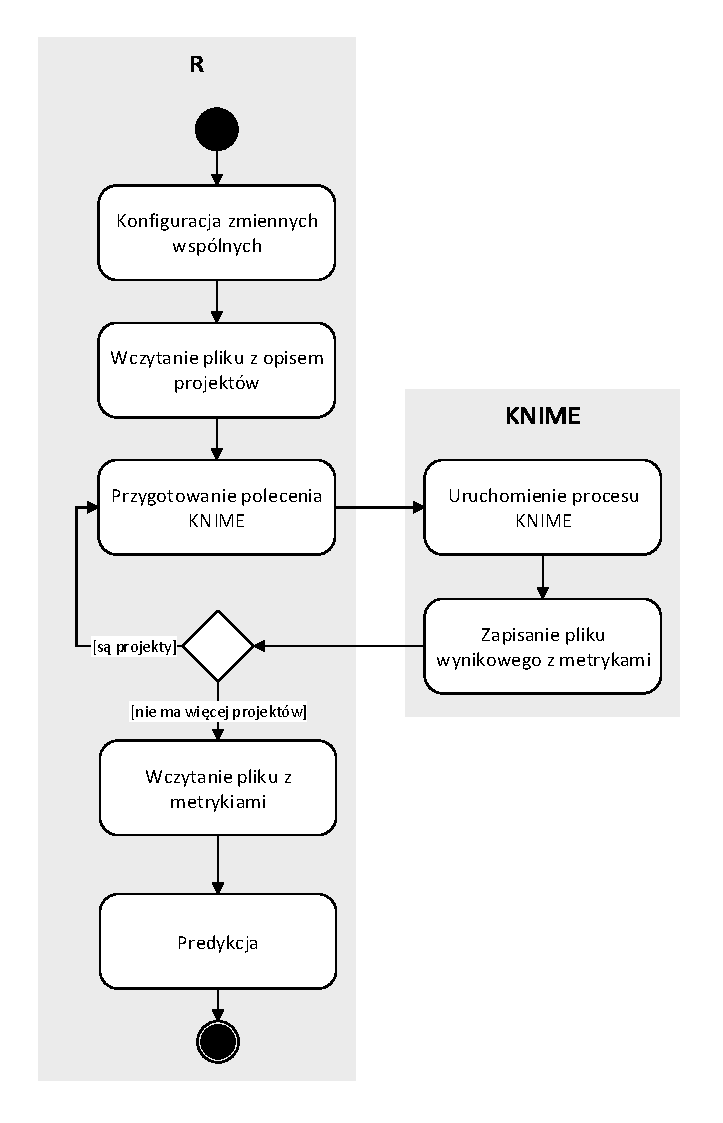
\includegraphics[width=0.5\textwidth]{diagrams/r-knime.pdf}
	\caption{Przebieg badania w �rodowisku R i KNIME}
	\label{r-knime}
\end{figure}

W tabeli \ref{wielkosc-projektow} zebrano dane dotycz�ce wielko�ci projekt�w oraz liczby b��d�w. Dane dotycz� wersji B~ka�dego projektu.

\begin{table}[htbp]
	\small
	\caption{Statystyki projekt�w}
	\label{wielkosc-projektow}
	\begin{center}
		\begin{tabular}{@{}lrrrrr@{}}
			\toprule
			\multirow{2}{*}{\bf Nazwa projektu} &
			\multirow{2}{*}{\bf LOC} &
			\bf Ilo�� &
			\bf Ilo�� &
			\bf B��dnych &
			\bf Udzia�
			\\
			&
			&
			\bf metod &
			\bf b��d�w &
			\bf metod &
			\bf b��dnych metod
			\\
			\midrule
			ECF                  & 54 264  & 9 306  & 290   & 236 & 2,54\% \\
			Ant                  & 60 715  & 9 120  & 480   & 407 & 4,46\% \\
			JMeter               & 50 181  & 7 592  & 447   & 365 & 4,81\% \\
			Commons Lang         & 15 802  & 2 555  & 37    & 34  & 1,33\% \\
			AspectJ              & 120 367 & 18 090 & 595   & 435 & 2,40\% \\
			CXF                  & 313 115 & 40 141 & 1 225 & 759 & 1,89\% \\
			Isis                 & 111 699 & 25 449 & 19    & 18  & 0,07\% \\
			Commons Email        & 1 202   & 210    & 13    & 9   & 4,29\% \\
			Commons JXPath       & 12 652  & 1 531  & 35    & 35  & 2,29\% \\
			Commons Logging      & 1 638   & 243    & 6     & 6   & 2,47\% \\
			Commons Net          & 5 536   & 1 169  & 94    & 78  & 6,67\% \\
			Accumulo             & 38 483  & 3 816  & 231   & 153 & 4,01\% \\
			Karaf                & 192 685 & 28 565 & 661   & 544 & 1,90\% \\
			ActiveMQ             & 66 861  & 10 582 & 116   & 102 & 0,96\% \\
			Hive                 & 104 202 & 15 254 & 381   & 296 & 1,94\% \\
			James Mailbox        & 14 258  & 2 130  & 20    & 20  & 0,94\% \\
			Jackrabbit FileVault & 25 861  & 3 344  & 55    & 34  & 1,02\% \\
			OpenJPA              & 174 748 & 36 954 & 1 378 & 944 & 2,55\% \\
			Jackrabbit Oak       & 116 458 & 14 971 & 983   & 731 & 4,88\% \\
			TomEE                & 9 535   & 1 091  & 63    & 56  & 5,13\% \\
			Tika                 & 31 166  & 3 797  & 226   & 212 & 5,58\% \\
			Lucene - Core        & 238 454 & 27 438 & 650   & 493 & 1,80\% \\
			Solr                 & 145 004 & 14 889 & 161   & 131 & 0,88\% \\
			Mahout               & 60 917  & 7 812  & 370   & 336 & 4,30\% \\
			Apache Gora          & 11 621  & 2 236  & 11    & 11  & 0,49\% \\
			Flume                & 40 956  & 4 791  & 115   & 107 & 2,23\% \\
			Nutch                & 15 013  & 1 776  & 122   & 89  & 5,01\% \\
			Apache Knox          & 25 857  & 3 359  & 23    & 22  & 0,65\% \\
			Phoenix              & 102 397 & 12 909 & 345   & 246 & 1,91\% \\
			\bottomrule
		\end{tabular}
	\end{center}
\end{table}


%%%%%%%%%%%%%%%%%%%%%%%%%%%%%%%%%%%%%%%%%%%%%%%%%%%%%%%%%%%%
\subsection{Om�wienie zebranych danych pomiarowych}

\noindent Zebrane dane zawieraj� 54 kolumny. Pierwsza zawiera sygnatur� metody, kolejne 50 to metryki wymienione w~rozdziale \ref{metryki}. S� to warto�ci liczbowe typu zmiennoprzecinkowego. Kolejne kolumny to: \textit{loc} zawieraj�ca miar� wielko�ci metody (warto�ci liczbowe ca�kowite), \textit{NumOfBugs} zawieraj�ca liczb� b��d�w (warto�ci liczbowe ca�kowite), \textit{Buggy} zawieraj�ca informacje o~tym czy metoda zawiera b��d czy nie (warto�ci \textit{1} lub \textit{0}). �adna z~kolumn nie zawiera nieokre�lonych lub brakuj�cych warto�ci.

Zebrano dane z~29 projekt�w o~otwartych �r�d�ach, w~dw�ch wersjach ka�dego projektu.

\paragraph{Wymagania dla repozytorium danych.} Dane powinny by� zgromadzone w~miejscu, kt�re umo�liwia �atwy dost�p poprzez protok� HTTP, bez uwierzytelniania lub logowania. Jest to istotne z~punktu widzenia wykorzystania narz�dzi do analizy i~przetwarzania tych danych. Pliki danych powinny by� oznaczone sumami kontrolnymi aby by�o mo�liwe sprawdzenie poprawno�ci ich pobierania.

\paragraph{Struktura danych i~zawarto�� zbioru.} Zbi�r metryk zosta� zaprojektowany w~celu umo�liwienia przechowywania danych z~projekt�w r�nego typu. Na najwy�szym poziomie zosta� podzielony na 2 grupy: projekty o~otwartym kodzie i~projekty w�asno�ciowe (odpowiednio katalogi \textit{open source} i~\textit{proprietary}). Katalog na kolejny poziomie zagnie�d�enia okre�la nazw� oprogramowania, a~wewn�trz znajduj� si� arkusze danych w~postaci plik�w CSV. CSV (ang. \textit{Comma-separated values}) jest to plik tekstowy rozdzielany przecinkami. Pliki z~danymi s� nazywane numerem/ nazw� wydania. W~przypadku repozytori�w Git zazwyczaj jest to nazwa tagu. W~pierwszej linii ka�dego pliku znajduj� si� nag��wki kolumn. W~tym samym katalogu co plik CSV powinien znajdowa� si� plik z~sum� kontroln� obliczon� funkcj� skr�tu MD5. Plik z~sum� kontroln� powinien mie� tak� sam� nazw� jak plik z~danymi, z~rozszerzeniem \textit{.md5}.

Na rysunku \ref{struktura-zbioru-danych} przedstawiono og�ln� struktur� zbioru danych wraz z~kilkoma przyk�adowymi projektami.

\begin{figure}[htbp]
	\centering
	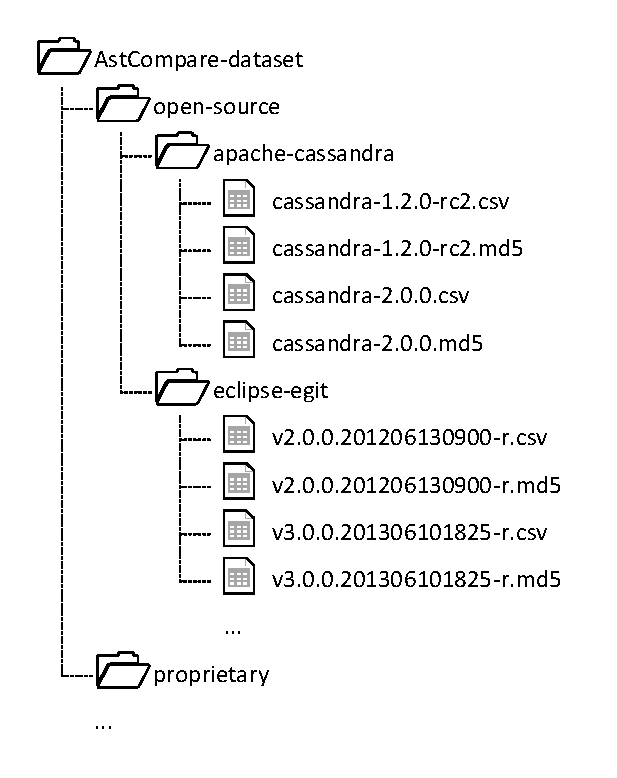
\includegraphics{diagrams/repozytorium-astcompare.pdf}
	\caption{Struktura repozytorium metryk AstMetrics}
	\label{struktura-zbioru-danych}
\end{figure}


%%%%%%%%%%%%%%%%%%%%%%%%%%%%%%%%%%%%%%%%%%%%%%%%%%%%%%%%%%%%
\chapter{Modele predykcji i ich ewaluacja}
\label{rozdzial4}
\noindent
\paragraph{LOC.} Przyj�to, �e podstawow� metod� wyszukiwania b��d�w, stanowi�c� punkt odniesienia, by�o przegl�danie kodu �r�d�owego od najmniejszej metody do najwi�kszej. Zatem sortuj�c dane wej�ciowe wed�ug kolumny \textit{LOC} niemalej�co mo�na obliczy� a~nast�pnie wykre�li� skuteczno�� takiego przegl�du. Wykresy na rysunku \ref{wedlug-loc} pokazuj�, �e jest to w~przybli�eniu zale�no�� liniowa, co udowadnia nisk� efektywno�� takich przegl�d�w. Taka metoda przegl�du b�dzie dalej nazywana \textit{LOC}.

\begin{figure}[htbp]
	\centering
	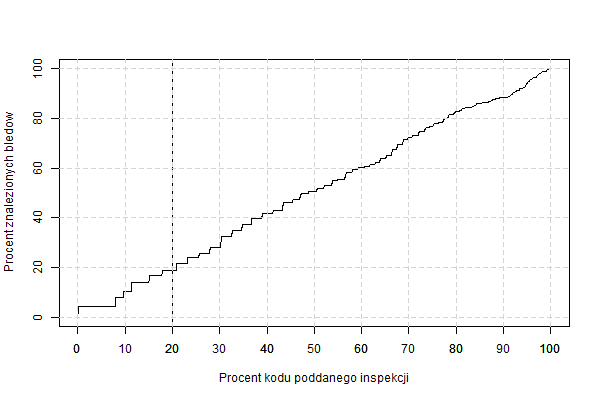
\includegraphics[width=0.49\textwidth]{charts/cost-ant-sorted}
	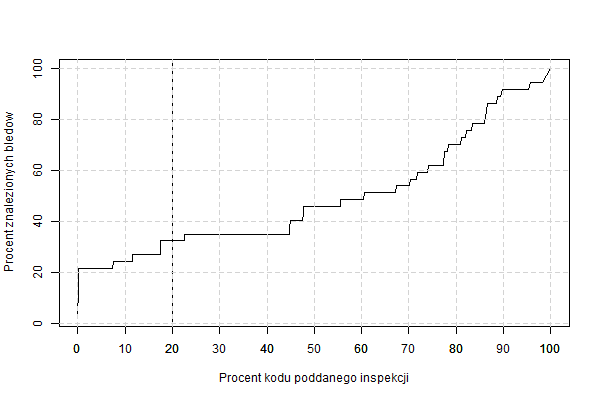
\includegraphics[width=0.49\textwidth]{charts/cost-commons-lang-sorted}
	\caption{Skuteczno�� przegl�du LOC dla projekt�w Ant i~Commons Lang}
	\label{wedlug-loc}
\end{figure}

\paragraph{Random Forest.} W~licznych badaniach, m.in. \cite{hata2012bug, kamei2010revisiting, lessmann2008benchmarking, liaw2002classification, mende2010effort} wykazano wysok� skuteczno�� metody Random Forest w~predykcji defekt�w. Ponadto udzia� metod z~b��dami jest niewielki, w~zwi�zku z~czym modele predykcji maj� tendencj� do klasyfikowania wszystkich element�w do klasy \textit{0}. Zauwa�ono takie zachowanie podczas stosowania regresji logistycznej w~\cite{hata2012bug}. Problem ten nie dotyka tej metody. Metoda Random Forest polega na tworzeniu du�ej liczby drzew decyzyjnych a~nast�pnie przypisaniu klasy na podstawie dominanty (najcz�stszej warto�ci) spo�r�d wszystkich wynik�w cz�ciowych.


W tabeli \ref{wyniki} zawarto wyniki predykcji z~u�yciem metody LOC oraz Random Forest. Wyniki powy�ej 60\% zaznaczono pogrubion� czcionk�. Uzyskane rezultaty potwierdzaj� wysok� skuteczno�� algorytmu Random Forest. W~kolejnej tabeli \ref{wyniki-rf} umieszczono wyniki pozosta�ych miar skuteczno�ci dla algorytmu Random Forest.

Metoda podstawowa (LOC) cechuje si� efektywno�ci� na poziomie �rednim 27,4\% ($\sigma=10,4$). Wynik uzyskany dla RandomForest wynosi �rednio 54,4\% ($\sigma=9,8$).

\begin{table}[htbp]
	\caption{Efektywno�� predykcji defekt�w pod wzgl�dem wysi�ku. Procent znalezionych b��d�w w~20\% kodu.}
	\label{wyniki}
	\begin{center}
		\tabcolsep=0.11cm
		\begin{tabular}{@{}lrr@{}}
			\toprule
			\bf Nazwa projektu &
			\bf LOC &
			\bf RandomForest
			\\
			\midrule
			ECF                  & 30 & \bf63 \\
			Ant                  & 19 & 49 \\
			JMeter               & 25 & \bf68 \\
			Commons Lang         & 32 & 49 \\
			AspectJ              & 18 & 59 \\
			CXF                  & 43 & 58 \\
			Isis                 & 26 & 32 \\
			Commons Email        & 15 & 54 \\
			Commons JXPath       & 34 & \bf60 \\
			Commons Logging      & 0  & 50 \\
			Commons Net          & 28 & 40 \\
			Accumulo             & 32 & \bf68 \\
			Karaf                & 24 & 43 \\
			ActiveMQ             & 19 & 55 \\
			Hive                 & 40 & 54 \\
			James Mailbox        & 35 & 50 \\
			Jackrabbit FileVault & 38 & \bf64 \\
			OpenJPA              & 34 & 50 \\
			Jackrabbit Oak       & 34 & \bf66 \\
			TomEE                & 19 & 41 \\
			Tika                 & 38 & 46 \\
			Lucene - Core        & 44 & 56 \\
			Solr                 & 43 & 50 \\
			Mahout               & 30 & 52 \\
			Apache Gora          & 9  & \bf64 \\
			Flume                & 18 & 46 \\
			Nutch                & 25 & \bf60 \\
			Apache Knox          & 17 & 52 \\
			Phoenix              & 24 & \bf69 \\
			\bottomrule
		\end{tabular}
	\end{center}
\end{table}



\begin{table}[htbp]
	\caption{Skuteczno�� predykcji defekt�w z~wykorzystaniem algorytmu Random Forest}
	\label{wyniki-rf}
	\begin{center}
		\begin{tabular}{@{}lS[table-format=1.3]S[table-format=1.3]S[table-format=1.3]@{}}
			\toprule
			\bf Nazwa projektu &
			\bf $A$ &
			\bf $\kappa$ &
			\bf $AUC$
			\\
			\midrule
			ECF                  & 0,985 & 0,594 & 0,760 \\
			Ant                  & 0,964 & 0,473 & 0,758 \\
			JMeter               & 0,971 & 0,639 & 0,815 \\
			Commons Lang         & 0,989 & 0,444 & 0,737 \\
			AspectJ              & 0,979 & 0,399 & 0,776 \\
			CXF                  & 0,975 & 0,255 & 0,795 \\
			Isis                 & 0,999 & 0,105 & 0,547 \\
			Commons Email        & 0,957 & 0,000 & 0,697 \\
			Commons JXPath       & 0,988 & 0,622 & 0,790 \\
			Commons Logging      & 0,971 & 0,447 & 0,767 \\
			Commons Net          & 0,941 & 0,320 & 0,757 \\
			Accumulo             & 0,960 & 0,466 & 0,829 \\
			Karaf                & 0,982 & 0,094 & 0,631 \\
			ActiveMQ             & 0,994 & 0,580 & 0,747 \\
			Hive                 & 0,982 & 0,130 & 0,691 \\
			James Mailbox        & 0,991 & 0,329 & 0,783 \\
			Jackrabbit FileVault & 0,990 & 0,057 & 0,637 \\
			OpenJPA              & 0,962 & 0,283 & 0,817 \\
			Jackrabbit Oak       & 0,962 & 0,488 & 0,817 \\
			TomEE                & 0,963 & 0,528 & 0,785 \\
			Tika                 & 0,960 & 0,425 & 0,693 \\
			Lucene - Core        & 0,973 & 0,288 & 0,760 \\
			Solr                 & 0,993 & 0,425 & 0,719 \\
			Mahout               & 0,969 & 0,450 & 0,747 \\
			Apache Gora          & 0,992 & 0,316 & 0,832 \\
			Flume                & 0,977 & 0,323 & 0,704 \\
			Nutch                & 0,967 & 0,582 & 0,788 \\
			Apache Knox          & 0,995 & 0,450 & 0,747 \\
			Phoenix              & 0,978 & 0,461 & 0,875 \\
			\bottomrule
		\end{tabular}
	\end{center}
\end{table}


Na kolejnych rysunkach zamieszczono wykresy krzywej efektywno�ci dla algorytmu Random Forest, dla pierwszych sze�ciu projekt�w. Im bardziej stroma jest krzywa efektywno�ci tym lepsza efektywno�� przeszukiwania kodu �r�d�owego.


\begin{figure}[htbp]
	\centering
	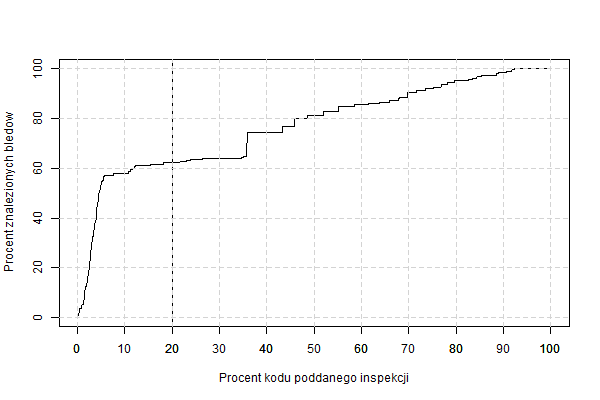
\includegraphics[width=.49\textwidth]{charts/cost-org-eclipse-ecf-rf}
	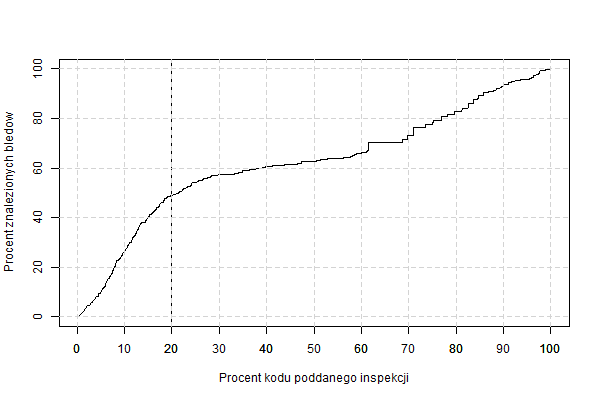
\includegraphics[width=.49\textwidth]{charts/cost-ant-rf}
	\caption{Krzywa efektywno�ci --- ECF i~Ant}
\end{figure}

\begin{figure}[htbp]
	\centering
	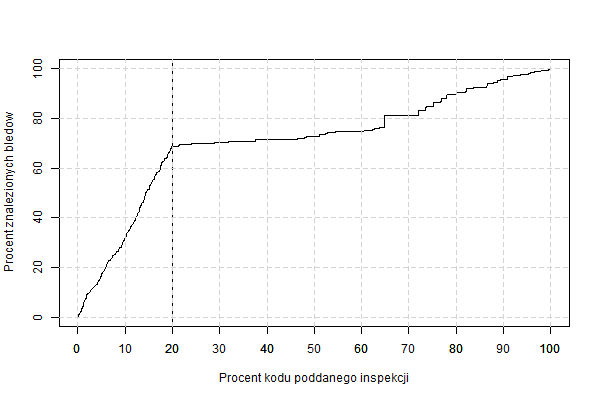
\includegraphics[width=.49\textwidth]{charts/cost-jmeter-rf}
	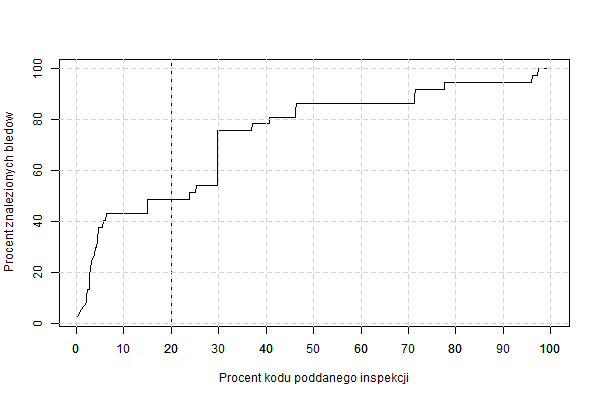
\includegraphics[width=.49\textwidth]{charts/cost-commons-lang-rf}
	\caption{Krzywa efektywno�ci --- JMeter i~Commons Lang}
\end{figure}

\begin{figure}[htbp]
	\centering
	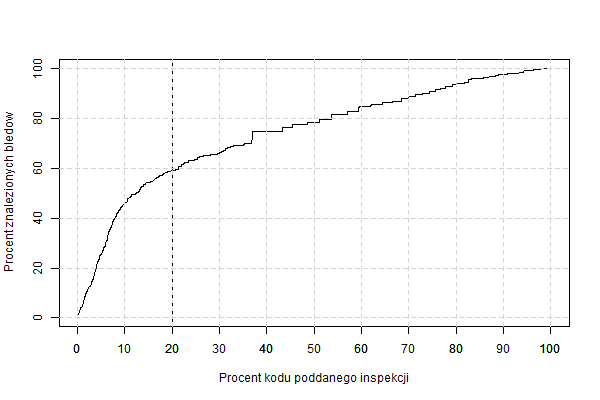
\includegraphics[width=.49\textwidth]{charts/cost-org-aspectj-rf}
	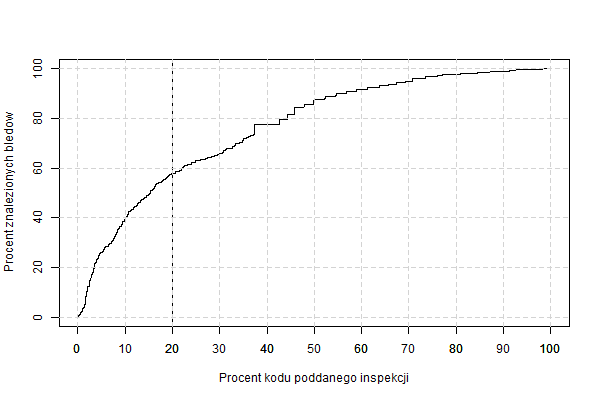
\includegraphics[width=.49\textwidth]{charts/cost-cxf-rf}
	\caption{Krzywa efektywno�ci --- AspectJ i~CXF}
\end{figure}

Tabele \ref{conf1} - \ref{conf3} zawieraj� macierze pomy�ek dla predykcji defekt�w w~poszczeg�lnych projektach z~wykorzystaniem algorytmu Random Forest.

\begin{table}[htbp]
	\caption{Macierz pomy�ek --- ECF i~Ant}
	\label{conf1}
	\begin{center}
		\begin{tabular}{|c|c|c|c|}
			\cline{3-4}
			\multicolumn{2}{c}{} & \multicolumn{2}{|c|}{przewidywany} \\
			\cline{3-4}
			\multicolumn{2}{c|}{} & 1 & 0 \\
			\cline{1-4}
			\multirow{2}{*}{rzeczywisty} & 1 	& 9060 & 131 \\
			\cline{2-4}
			& 0 								& 10 & 105 \\
			\cline{1-4}
		\end{tabular}
		~
		\begin{tabular}{|c|c|c|c|}
			\cline{3-4}
			\multicolumn{2}{c}{} & \multicolumn{2}{|c|}{przewidywany} \\
			\cline{3-4}
			\multicolumn{2}{c|}{} & 1 & 0 \\
			\cline{1-4}
			\multirow{2}{*}{rzeczywisty} & 1 	& 8642 & 255 \\
			\cline{2-4}
			& 0 								& 71 & 152 \\
			\cline{1-4}
		\end{tabular}
	\end{center}
\end{table}

\begin{table}[htbp]
	\caption{Macierz pomy�ek --- JMeter i~Commons Lang}
	\label{conf2}
	\begin{center}
		\begin{tabular}{|c|c|c|c|}
			\cline{3-4}
			\multicolumn{2}{c}{} & \multicolumn{2}{|c|}{przewidywany} \\
			\cline{3-4}
			\multicolumn{2}{c|}{} & 1 & 0 \\
			\cline{1-4}
			\multirow{2}{*}{rzeczywisty} & 1 	& 208 & 57 \\
			\cline{2-4}
			& 0 								& 157 & 7170 \\
			\cline{1-4}
		\end{tabular}
		~
		\begin{tabular}{|c|c|c|c|}
			\cline{3-4}
			\multicolumn{2}{c}{} & \multicolumn{2}{|c|}{przewidywany} \\
			\cline{3-4}
			\multicolumn{2}{c|}{} & 1 & 0 \\
			\cline{1-4}
			\multirow{2}{*}{rzeczywisty} & 1 	& 11 & 2 \\
			\cline{2-4}
			& 0 								& 23 & 2519 \\
			\cline{1-4}
		\end{tabular}
	\end{center}
\end{table}

\begin{table}[htbp]
	\caption{Macierz pomy�ek --- AspectJ i~CXF}
	\label{conf3}
	\begin{center}
		\begin{tabular}{|c|c|c|c|}
			\cline{3-4}
			\multicolumn{2}{c}{} & \multicolumn{2}{|c|}{przewidywany} \\
			\cline{3-4}
			\multicolumn{2}{c|}{} & 1 & 0 \\
			\cline{1-4}
			\multirow{2}{*}{rzeczywisty} & 1 	& 134 & 72 \\
			\cline{2-4}
			& 0 								& 301 & 17583 \\
			\cline{1-4}
		\end{tabular}
		~
		\begin{tabular}{|c|c|c|c|}
			\cline{3-4}
			\multicolumn{2}{c}{} & \multicolumn{2}{|c|}{przewidywany} \\
			\cline{3-4}
			\multicolumn{2}{c|}{} & 1 & 0 \\
			\cline{1-4}
			\multirow{2}{*}{rzeczywisty} & 1 	& 182 & 409 \\
			\cline{2-4}
			& 0 								& 577 & 38973 \\
			\cline{1-4}
		\end{tabular}
	\end{center}
\end{table}


%%%%%%%%%%%%%%%%%%%%%%%%%%%%%%%%%%%%%%%%%%%%%%%%%%%%%%%%%%%%
\chapter{Podsumowanie}
\label{rozdzial5}
\noindent
\paragraph{Trudno�ci podczas realizacji pracy.} Podczas uruchamiania oblicze� zaplanowanych do wykonania w ramach projektu, okaza�o si�, �e czas przetwarzania na �redniej klasy komputerze osobistym jest zdecydowanie zbyt d�ugi. Po wykonaniu cz�ci oblicze� i zebraniu danych z 6 projekt�w zdecydowano o przeniesieniu wykonania programu do chmury obliczeniowej. Uruchomiono instacj� maszyny wirtualnej w chmurze Windows Azure. Niezb�dne by�o uruchomienie instancji dysponuj�cej odpowiedni� ilo�ci� pami�ci operacyjnej, przydzielono 14 GB pami�ci RAM, z czego 4 GB przeznaczono na przechowywanie plik�w na wirtualnym dysku RAM.

Kolejnym wyzwaniem napotkanym w trakcie tworzenia rozwi�zania by�o wykorzystanie wtyczek z pakietu DePress w �rodowisku KNIME, pomimo przeprowadzenia predykcji i oblicze� statystycznych w �rodowisku R. Dzi�ki wykorzystaniu trybu wsadowego KNIME uzyskano zadowalaj�cy rezultat, daj�cy mo�liwo�� automatycznego przeprowadzenia oblicze�. Wymagane do tego jest jednak zainstalowanie KNIME oraz wtyczek z pakietu DePress.



\paragraph{Zagro�enia dla wiarygodno�ci.} Istniej� zagro�enia dla wiarygodno�ci przeprowadzonego badania. Metoda wyszukiwania b��d�w bazuje na zg�oszeniach w systemie kontroli wersji oraz opisach rewizji w systemie wersjonowania kodu. Od jako�ci tych danych zale�y jako�� uzyskanych informacji o b��dach w kodzie �r�d�owym. Cz�� b��d�w mog�a zosta� �le opisana przez co niemo�liwe by�o dopasowanie rewizji do zg�oszonego b��du. Z drugiej strony cz�� zg�oszonych b��d�w mo�e nie by� b��dami, co tak�e wp�ywa na niedoskona�o�� zebranych danych.

Filtrowanie danych wej�ciowych tak�e mo�e by� nieprecyzyjne. Opracowano rozi�zanie bazuj�ce na wy��czaniu okre�lonego jednego katalogu (razem z podkatalogami), co mo�e by� niewystarczaj�ce ze wzgl�du na uk�ad zawarto�ci niekt�rych repozytori�w.



\paragraph{Podsumowanie.} Stworzone modele predykcji defekt�w na poziomie metod charakteryzuj� si� wysok� skuteczno�ci�. Dzi�ki wykorzystaniu du�ej liczby metryk procesu oraz odpowiedniego algorytmu klasyfikacji, mo�na znacz�co ograniczy� koszty przegl�du kodu, co z~kolei pozwala na ograniczenie koszt�w zapewnienia jako�ci w~procesie tworzenia oprogramowania. Uzyskane wyniki daj� podstawy do pozytywnej oceny stworzonych modeli predykcji. Dzi�ki zastosowaniu opracowanej metody w procesie wytwarzania oprogramowania, czas zaoszcz�dzony na pe�nych przegl�dach kodu, mo�na przeznaczy� na inne zadania realizowane przez zesp� programist�w i tester�w.

W ramach niniejszej pracy dyplomowej stworzono r�wnie� wtyczk� KNIME s�u��c� do wyliczenia metryk procesu AST (AstMetrics). Zbudowano te� repozytorium metryk oraz zebrano metryki z~29 projekt�w. Pozyskane dane mog� pos�u�y� do budowania i~ewaluacji nowych modeli predykcji w~celu uzyskania jeszcze lepszych rezultat�w. Repozytorium metryk opublikowano pod adresem\\https://github.com/mkutyba/AstMetrics-dataset.



\paragraph{Propozycja dalszych bada�.} Zauwa�ono mo�liwo�ci dalszego rozwoju badania w celu osi�gni�cia wi�kszej efektywno�ci. Mo�na dokona� wst�pnej obr�bki zmiennych wej�ciowych, np. stosuj�c metody nadpr�bkowania lub podpr�bkowania albo przefiltrowa� predyktory wy��czaj�c te, kt�re maj� wariancj� blisk� zeru (sta�� warto��), s� skorelowane, lub w inny spos�b.


%%%%%%%%%%%%%%%%%%%%%%%%%%%%%%%%%%%%%%%%%%%%%%%%%%%%%%%%%%%%





 
%\listoffigures
%\listoftables

\bibliographystyle{iisthesis}
\bibliography{bibliografia}

%\appendix
%\chapter{Co� dodatkowego}
%\pagestyle{plain}

\end{document}
